% ============================================================
%  REVISTA MECATRÓNICA — DOCUMENTO MAESTRO UNIFICADO
%  Orden:
%   1.  Portada
%   2.  Índice
%   3.  Introducción + UASLP   (Oscar / intro)
%   4.  Talleres
%   5.  Historia y Aplicaciones
%   6.  Editorial: El ADN del Ingeniero
%   7.  Entrevista Dr. Víctor Espinosa
%   8.  Entrevista Dr. Martínez Montejano (versión compacta)
%   9.  Entrevista Dr. Germánico González
%  10.  Entrevista Benny
%  11.  Entrevista Gael
%  12.  Mecatrónica en Números (comparativa fondo claro)
%  13.  Entrevista Lázaro
%  14.  Entrevista Erick Moreno Negrete
%  15.  Entrevista Mtra. Ivana López Reina
%  16.  Conclusiones + Referencias
% ============================================================
\documentclass[10pt]{article}

% ── Página base (páginas interiores con márgenes) ────────────
\usepackage[a4paper,
            top=2.2cm, bottom=2.0cm,
            left=2.0cm, right=2.0cm,
            headheight=16pt]{geometry}

% ── Tipografía ───────────────────────────────────────────────
\usepackage[T1]{fontenc}
\usepackage[utf8]{inputenc}
\usepackage{helvet}
\renewcommand{\familydefault}{\sfdefault}
\usepackage{microtype}

% ── Color — paleta completa de la revista ────────────────────
\usepackage[dvipsnames,svgnames,x11names]{xcolor}
\definecolor{fondoOscuro}{HTML}{0D1117}
\definecolor{azulOscuro}{HTML}{1B3A5C}
\definecolor{naranja}{HTML}{E87722}
\definecolor{naranjaClaro}{HTML}{FDF0E6}
\definecolor{blanco}{HTML}{FFFFFF}
\definecolor{grisTexto}{HTML}{CCCCCC}
\definecolor{lineaGris}{HTML}{2A3A4A}
\definecolor{grisClaro}{HTML}{1E2A38}
\definecolor{verdeTech}{HTML}{1A3A2A}
\definecolor{verdeAccento}{HTML}{2ECC71}
\definecolor{fondoClaro}{HTML}{F0EDE8}
\definecolor{textoOscuro}{HTML}{1A1A2E}
\definecolor{textoGris}{HTML}{3A3A5A}
\definecolor{lineaAzul}{HTML}{A8C4DC}
\definecolor{azulClaro}{HTML}{E8F0F8}
\definecolor{azulCelda}{HTML}{162436}
\definecolor{cyan}{HTML}{2EC4B6}
\definecolor{ambar}{HTML}{F0A500}
\definecolor{ambarClaro}{HTML}{FFF8E7}
\definecolor{ambarFondo}{HTML}{2A2010}
\definecolor{cian}{HTML}{00B4D8}
\definecolor{cianSuave}{HTML}{023E54}
\definecolor{cianMedio}{HTML}{0D3D52}
\definecolor{rose}{HTML}{C0392B}
\definecolor{roseFondo}{HTML}{1E0A09}
\definecolor{viola}{HTML}{8B5CF6}
\definecolor{violaOscuro}{HTML}{1A0D33}
\definecolor{violaFondo}{HTML}{120820}
\definecolor{violaMedio}{HTML}{2D1B52}
% Colores rose — entrevista Mtra. Ivana
\definecolor{roseMedio}{HTML}{C0392B}
\definecolor{roseFondo}{HTML}{1E0A09}
\definecolor{roseOscuro}{HTML}{150504}
% Redefine rose con tono más vivo para Ivana
\definecolor{rose}{HTML}{FF6B55}

% ── Paquetes ─────────────────────────────────────────────────
\usepackage{multicol}
\usepackage{tcolorbox}
\tcbuselibrary{skins,breakable}
\usepackage{graphicx}
\usepackage{tikz}
\usetikzlibrary{calc,shapes.geometric}
\usepackage{eso-pic}
\usepackage{ragged2e}
\usepackage{array}
\usepackage{booktabs}
\usepackage{tabularx}
\usepackage{colortbl}
\usepackage{amssymb}
\usepackage{titlesec}
\usepackage{fancyhdr}
\usepackage{enumitem}
\usepackage{hyperref}
\usepackage{float}
\usepackage{caption}
\usepackage[pages=some]{background}

\hypersetup{colorlinks=true, urlcolor=naranja, linkcolor=azulOscuro,
            pdfborder={0 0 0}}

\setlength{\parskip}{3pt}
\setlength{\parindent}{0pt}
\setlength{\columnsep}{14pt}

% ── Fondo imagen para páginas intro (background package) ─────
\backgroundsetup{
  scale=1, opacity=0.12, angle=0,
  contents={\includegraphics[
    width=\paperwidth, height=\paperheight]{ofimatica/fondo.jpeg}}}

% ── Encabezado/pie páginas interiores ────────────────────────
\pagestyle{fancy}
\fancyhf{}
\fancyhead[LE,RO]{\small\color{textoGris}\thepage}
\fancyhead[RE,LO]{%
  \small\color{azulOscuro}\textbf{INGENIERÍA MECATRÓNICA}%
  \color{textoGris}\ |\ Edición Especial 2026}
\fancyfoot[C]{\footnotesize\color{textoGris}%
  Universidad Autónoma de San Luis Potosí}
\renewcommand{\headrulewidth}{0pt}
\fancyhead[C]{%
  \begin{tikzpicture}[remember picture,overlay]
    \draw[naranja, line width=1.2pt]
      ([yshift=-0.30cm]current page.north west)
      -- ([yshift=-0.30cm]current page.north east);
  \end{tikzpicture}}

% ── Estilos de sección ───────────────────────────────────────
\titleformat{\section}
  {\color{naranja}\fontsize{14}{17}\selectfont\bfseries}
  {}{0em}{}[{\color{naranja}\titlerule[1.2pt]}]
\titlespacing{\section}{0pt}{10pt}{5pt}

\titleformat{\subsection}
  {\color{azulOscuro}\normalsize\bfseries}
  {}{0em}{}[{\color{lineaAzul}\titlerule[0.5pt]}]
\titlespacing{\subsection}{0pt}{7pt}{4pt}

% ════════════════════════════════════════════════════════════
%  COMANDOS GLOBALES
% ════════════════════════════════════════════════════════════

\newcommand{\tagLabel}[2]{%
  \colorbox{#1}{\textcolor{blanco}%
    {\fontsize{6}{7}\selectfont\bfseries\quad#2\quad}}}

\newcommand{\lineaNaranja}{%
  \noindent{\color{naranja}\rule{\linewidth}{1.5pt}}\par\vspace{3pt}}
\newcommand{\lineaVerde}{%
  \noindent{\color{verdeAccento}\rule{\linewidth}{1.5pt}}\par\vspace{3pt}}
\newcommand{\lineaAmbar}{%
  \noindent{\color{ambar}\rule{\linewidth}{1.5pt}}\par\vspace{3pt}}
\newcommand{\lineaCian}{%
  \noindent{\color{cian}\rule{\linewidth}{1.5pt}}\par\vspace{3pt}}
\newcommand{\lineaViola}{%
  \noindent{\color{viola}\rule{\linewidth}{1.5pt}}\par\vspace{2pt}}
\newcommand{\lineaGrisH}{%
  \noindent{\color{lineaGris}\rule{\linewidth}{0.4pt}}\par}
\newcommand{\lineaGrisHc}{%
  \noindent{\color{lineaAzul}\rule{\linewidth}{0.5pt}}\par}
\newcommand{\lineaCyanT}{%
  \noindent{\color{cyan}\rule{\linewidth}{1.2pt}}\par}

% Preguntas/respuestas (múltiples estilos)
\newcommand{\preguntaN}[1]{%   naranja con cuadrado
  \vspace{4pt}{\small\bfseries\color{naranja}%
  \raisebox{0.5pt}{\tiny$\blacksquare$}\enspace#1}\par}
\newcommand{\preguntaV}[1]{%   verde
  \vspace{3pt}{\footnotesize\bfseries\color{verdeAccento}P: #1}\par}
\newcommand{\preguntaA}[1]{%   ámbar con cuadrado TikZ
  \vspace{3pt}%
  \noindent
  
\begin{tikzpicture}[baseline=(T.base)]
    \node[fill=ambar, inner sep=2pt,
          minimum width=6pt, minimum height=6pt] (T) {};
  \end{tikzpicture}\,%
  {\footnotesize\bfseries\color{ambar}#1}\par}

% Contador para preguntas cian numeradas
\newcounter{qnum}
\newcommand{\resetQ}{\setcounter{qnum}{0}}
\newcommand{\preguntaC}[1]{%   cian numerada
  \stepcounter{qnum}%
  \vspace{3pt}%
  \noindent
  \colorbox{cian}{\textcolor{fondoOscuro}{%
    \fontsize{6}{6}\selectfont\bfseries\ \theqnum\ }}%
  \hspace{2pt}{\footnotesize\bfseries\color{cian}#1}\par}

\newcommand{\respuesta}[1]{%
  {\small\color{grisTexto}#1}\par\vspace{2pt}}
\newcommand{\respuestaS}[1]{%  pequeña
  {\footnotesize\color{grisTexto}#1}\par\vspace{1pt}}
\newcommand{\respuestaV}[1]{%  verde
  {\footnotesize\color{grisTexto}\textbf{R:} #1}\par}
\newcommand{\itemBullet}[1]{%
  \vspace{2pt}\noindent
  \textcolor{naranja}{\small$\blacktriangleright$}\,%
  {\small\color{textoGris}#1}\par}
\newcommand{\itemSidebar}[1]{%
  \vspace{1pt}\noindent
  \textcolor{naranja}{\small$\blacksquare$}\,%
  {\footnotesize\color{grisTexto}#1}\par}
\newcommand{\itemSidebarV}[1]{%
  \vspace{2pt}\noindent
  \textcolor{verdeAccento}{\small$\blacktriangleright$}\,%
  {\footnotesize\color{grisTexto}#1}\par}
\newcommand{\itemC}[1]{%
  \vspace{2pt}\noindent
  \textcolor{cian}{\small$\blacktriangleright$}\,%
  {\footnotesize\color{grisTexto}#1}\par}
\newcommand{\itemPerfil}[2]{%
  \vspace{3pt}%
  \noindent{\fontsize{6}{7.5}\selectfont\bfseries\color{viola}%
    \MakeUppercase{#1}}\par
  \noindent{\fontsize{7.5}{9.5}\selectfont\color{grisTexto}#2}\par}
\newcommand{\itemPerfilA}[2]{%
  \vspace{3pt}%
  \noindent{\fontsize{6.5}{8}\selectfont\bfseries\color{ambar}%
    \MakeUppercase{#1}}\par
  \noindent{\fontsize{7.5}{9.5}\selectfont\color{blanco}#2}\par}

\newcommand{\barraAccento}{%
  \noindent\colorbox{naranja}{\hspace{2.8cm}\rule{0pt}{6pt}}\par\vspace{4pt}}

\newcommand{\encabezadoCol}[2]{%
  \vspace{2pt}%
  \noindent\colorbox{naranja}{\textcolor{blanco}{\footnotesize\bfseries\ #1\ }}%
  \hspace{3pt}{\small\bfseries\color{blanco}#2}\par
  \vspace{2pt}%
  \noindent{\color{naranja}\rule{\linewidth}{0.8pt}}\par\vspace{4pt}}

% Foto de entrevistado — busca en carpeta 
% Uso inline: \fotoPersona{nombre.jpg}{4.0cm}{4.5cm}
\newcommand{\fotoPersona}[3]{%
  \IfFileExists{#1}{%
    \includegraphics[width=#2, height=#3, keepaspectratio]{#1}%
  }{%
    \begin{tikzpicture}
      \fill[grisClaro] (0,0) rectangle (#2,#3);
      \draw[naranja, line width=1pt] (0,0) rectangle (#2,#3);
      \node[blanco, font=\tiny\bfseries, align=center]
        at (#2/2,#3/2) {FOTO};
    \end{tikzpicture}%
  }}

% Foto en caja tcolorbox (para perfiles con marco de color)
% Uso: \fotoEnCaja{nombre.jpg}{ancho}{alto}{color marco}
\newcommand{\fotoEnCaja}[4]{%
  \IfFileExists{#1}{%
    \includegraphics[width=#2, height=#3, keepaspectratio]{#1}%
  }{%
    \begin{tikzpicture}
      \fill[grisClaro] (0,0) rectangle (#2,#3);
      \draw[#4, line width=1.2pt] (0,0) rectangle (#2,#3);
      \node[blanco, font=\tiny\bfseries, align=center]
        at (#2/2,#3/2) {FOTO};
    \end{tikzpicture}%
  }}

% Compatibilidad: fotoSimulada → fotoEnCaja con placeholder siempre
\newcommand{\fotoSimulada}[3]{%
  \begin{tikzpicture}
    \fill[grisClaro] (0,0) rectangle (#1,#2);
    \draw[#3, line width=1.5pt] (0,0) rectangle (#1,#2);
    \node[blanco, font=\small\bfseries, align=center]
      at (#1/2,#2/2) {FOTO};
  \end{tikzpicture}}

% ── Comandos rose — Mtra. Ivana ──────────────────────────────
\newcommand{\lineaRose}{%
  \noindent{\color{rose}\rule{\linewidth}{1.5pt}}\par\vspace{3pt}}

\newcommand{\preguntaR}[1]{%
  \stepcounter{qnum}%
  \vspace{3pt}%
  \noindent
  \colorbox{rose}{\textcolor{fondoOscuro}{%
    \fontsize{6}{6}\selectfont\bfseries\ \theqnum\ }}%
  \hspace{2pt}{\footnotesize\bfseries\color{rose}#1}\par}

\newcommand{\itemSidebarR}[1]{%
  \vspace{1pt}\noindent
  \textcolor{rose}{\small$\blacksquare$}\,%
  {\footnotesize\color{grisTexto}#1}\par}

\newcommand{\itemCR}[1]{%
  \vspace{2pt}\noindent
  \textcolor{rose}{\small$\blacktriangleright$}\,%
  {\footnotesize\color{grisTexto}#1}\par}

\newcommand{\itemPerfilR}[2]{%
  \vspace{3pt}%
  \noindent{\fontsize{6}{7.5}\selectfont\bfseries\color{rose}%
    \MakeUppercase{#1}}\par
  \noindent{\fontsize{7.5}{9.5}\selectfont\color{grisTexto}#2}\par}


\newcommand{\fotoRevista}[3][0.42\linewidth]{%
  \begin{figure}[H]\centering
    \includegraphics[width=#1]{#2}
    \captionsetup{font={small,color=textoGris},
      labelfont={bf,color=naranja},labelsep=quad}
    \caption{#3}
  \end{figure}}

\newcommand{\tabHead}[1]{{\fontsize{7.5}{9}\selectfont\bfseries\color{blanco}#1}}
\newcommand{\tabCell}[1]{{\fontsize{7.5}{9}\selectfont\color{textoGris}#1}}
\newcommand{\tabCellB}[1]{{\fontsize{7.5}{9}\selectfont\bfseries\color{textoOscuro}#1}}

\newcommand{\tarjetaPersona}[4]{%
  \begin{tcolorbox}[colback=grisClaro,colframe=#1,
    arc=0pt,boxrule=1pt,left=6pt,right=6pt,top=5pt,bottom=5pt]
  \noindent{\color{#1}\rule{\linewidth}{2pt}}\par\vspace{3pt}
  {\fontsize{8}{10}\selectfont\bfseries\color{blanco}#2}\par\vspace{1pt}
  {\fontsize{6.5}{8}\selectfont\color{#1}#3}\par\vspace{3pt}
  \hfill{\fontsize{6}{7}\selectfont\color{lineaGris}p.\ #4}%
  \end{tcolorbox}\vspace{5pt}}

\newcommand{\tarjetaQA}[3]{%
  \begin{tcolorbox}[colback=violaFondo,colframe=#1,
    arc=0pt,boxrule=0.8pt,left=6pt,right=6pt,top=5pt,bottom=5pt,
    before=\vspace{3pt},after=\vspace{0pt}]
  {\fontsize{6.5}{8}\selectfont\bfseries\color{#1}%
    \raisebox{0.3pt}{\tiny$\blacksquare$}\enspace PREGUNTA}\par
  \vspace{2pt}
  {\fontsize{7.5}{9}\selectfont\bfseries\color{blanco}#2}\par
  \vspace{3pt}
  {\color{viola!40}\rule{\linewidth}{0.3pt}}\par\vspace{2pt}
  {\fontsize{6.8}{8.5}\selectfont\color{grisTexto}#3}
  \end{tcolorbox}}

% ── Ambientes de cajas ───────────────────────────────────────
\newenvironment{cajaDato}[1]{%
  \begin{tcolorbox}[colback=naranjaClaro,colframe=naranja,
    arc=0pt,boxrule=1pt,title={\small\bfseries\color{naranja}#1},
    coltitle=naranja,
    attach boxed title to top left={yshift=-2mm,xshift=4mm},
    boxed title style={colback=blanco,colframe=naranja,arc=0pt,boxrule=0.8pt},
    left=7pt,right=7pt,top=9pt,bottom=6pt]
  \small\color{textoGris}\RaggedRight}{\end{tcolorbox}}

\newenvironment{cajaAzul}[1]{%
  \begin{tcolorbox}[colback=azulClaro,colframe=azulOscuro,
    arc=0pt,boxrule=1pt,left=7pt,right=7pt,top=6pt,bottom=6pt]
  \noindent{\small\bfseries\color{azulOscuro}#1}\par
  \noindent{\color{azulOscuro}\rule{\linewidth}{0.6pt}}\par\vspace{3pt}%
  \small\color{textoGris}\RaggedRight}{\end{tcolorbox}}

\newenvironment{cajaTaller}[1]{%
  \begin{tcolorbox}[colback=verdeTech,colframe=verdeAccento,
    arc=0pt,boxrule=1pt,left=7pt,right=7pt,top=6pt,bottom=6pt]
  \noindent{\small\bfseries\color{verdeAccento}#1}\par
  \noindent{\color{verdeAccento}\rule{\linewidth}{0.5pt}}\par\vspace{3pt}%
  \small\color{grisTexto}\RaggedRight}{\end{tcolorbox}}

\newenvironment{cajaProyectoV}{%
  \begin{tcolorbox}[colback=verdeTech,colframe=verdeAccento,
    arc=0pt,boxrule=1pt,left=8pt,right=8pt,top=6pt,bottom=6pt]}%
  {\end{tcolorbox}}

\newenvironment{citaRevista}{%
  \begin{tcolorbox}[colback=azulOscuro,colframe=naranja,
    arc=0pt,boxrule=1.2pt,left=8pt,right=8pt,top=6pt,bottom=6pt]
  \centering\small\bfseries\color{blanco}CITA DESTACADA:\par
  \vspace{3pt}\itshape\normalsize\color{grisTexto}}{\end{tcolorbox}}

\newenvironment{citaDestacada}{%
  \begin{tcolorbox}[colback=fondoOscuro,colframe=blanco,
    arc=0pt,boxrule=1.2pt,left=6pt,right=6pt,top=5pt,bottom=5pt]
  \centering\bfseries\color{blanco}\small
  CITA DESTACADA:\par\vspace{3pt}\itshape\normalsize}{\end{tcolorbox}}

\newenvironment{citaDatoClave}{%
  \begin{tcolorbox}[colback=fondoOscuro,colframe=blanco,
    arc=0pt,boxrule=1.2pt,left=6pt,right=6pt,top=5pt,bottom=5pt]
  \centering\bfseries\color{blanco}\small
  DATO CLAVE:\par\vspace{3pt}\itshape\normalsize}{\end{tcolorbox}}

\newenvironment{citaCian}{%
  \begin{tcolorbox}[colback=cianMedio,colframe=cian,
    arc=0pt,boxrule=1.2pt,left=7pt,right=7pt,top=5pt,bottom=5pt]
  \centering\fontsize{7}{8}\selectfont\bfseries\color{cian}
  CITA DESTACADA:\par\vspace{3pt}\itshape\footnotesize\color{grisTexto}}%
  {\end{tcolorbox}}

\newenvironment{sidebar}[1]{%
  \begin{tcolorbox}[colback=grisClaro,colframe=grisClaro,
    arc=0pt,boxrule=0pt,left=6pt,right=6pt,top=5pt,bottom=5pt]
  \noindent{\small\bfseries\color{naranja}#1}\par
  \noindent{\color{naranja}\rule{\linewidth}{1pt}}\par\vspace{3pt}}%
  {\end{tcolorbox}}

\newenvironment{sidebarAzul}[1]{%
  \begin{tcolorbox}[colback=azulOscuro,colframe=azulOscuro,
    arc=0pt,boxrule=0pt,left=6pt,right=6pt,top=5pt,bottom=5pt]
  \noindent{\small\bfseries\color{blanco}#1}\par
  \noindent{\color{naranja}\rule{\linewidth}{1pt}}\par\vspace{2pt}}%
  {\end{tcolorbox}}

\newenvironment{bloqueNaranja}[1]{%
  \begin{tcolorbox}[colback=naranjaClaro,colframe=naranja,
    arc=0pt,boxrule=1.2pt,left=7pt,right=7pt,top=6pt,bottom=6pt]
  \noindent{\footnotesize\bfseries\color{naranja}\MakeUppercase{#1}}\par
  \noindent{\color{naranja}\rule{\linewidth}{0.6pt}}\par\vspace{3pt}%
  \footnotesize\color{textoGris}\RaggedRight}{\end{tcolorbox}}

\newenvironment{bloqueQ}[2]{%
  \begin{tcolorbox}[colback=cianSuave,colframe=#1,
    arc=0pt,boxrule=1.2pt,left=8pt,right=8pt,top=6pt,bottom=6pt,
    title={\fontsize{7.5}{9}\selectfont\bfseries\color{blanco}\MakeUppercase{#2}},
    coltitle=blanco,
    attach boxed title to top left={yshift=-2.5mm,xshift=6pt},
    boxed title style={colback=#1,colframe=#1,arc=0pt,boxrule=0pt,
      left=4pt,right=4pt,top=2pt,bottom=2pt}]}%
  {\end{tcolorbox}}

% ── Caption global ───────────────────────────────────────────
\captionsetup{font={small,color=textoGris},
              labelfont={bf,color=naranja},labelsep=quad}

% ── Macro: pie estándar páginas full-bleed ───────────────────
\newcommand{\pieRevista}[2]{%
  \vspace*{\fill}\vspace{3pt}%
  \lineaGrisH\vspace{3pt}%
  {\footnotesize%
    \colorbox{azulOscuro}{\textcolor{blanco}{\footnotesize\textbf{\quad[R]\quad}}}\,%
    \textcolor{blanco}{\textbf{REVISTA MECATR\'ONICA}}\hfill
    \textcolor{grisTexto}{MARZO 2026\quad}%
    \textcolor{#1}{\textbf{#2}}}}

% ════════════════════════════════════════════════════════════
\begin{document}

% ────────────────────────────────────────────────────────────
% PÁG. 1 — PORTADA
% ────────────────────────────────────────────────────────────
\clearpage
\newgeometry{margin=0cm}
\pagestyle{empty}
\noindent\includegraphics[width=\paperwidth,height=\paperheight]{portada1.jpeg}
\clearpage
\restoregeometry
\pagestyle{fancy}

% ────────────────────────────────────────────────────────────
% PÁG. 2 — ÍNDICE
% ────────────────────────────────────────────────────────────
\clearpage
{
  % Estilo local del índice
  \renewcommand{\contentsname}{%
    {\color{naranja}\fontsize{20}{24}\selectfont\bfseries
     CONTENIDO\par}%
    {\color{naranja}\rule{\linewidth}{1.5pt}}\par\vspace{4pt}}
  \hypersetup{linkcolor=azulOscuro}
  \setlength{\columnsep}{20pt}
  \tableofcontents
}
\clearpage

% ════════════════════════════════════════════════════════════
% SECCIÓN 1 — INTRODUCCIÓN + UASLP + TALLERES  (págs. 3–5)
% ════════════════════════════════════════════════════════════
\addcontentsline{toc}{section}{Introducción a la Mecatrónica y la UASLP}
\BgThispage

\noindent
\tagLabel{naranja}{FUNDAMENTOS}\hspace{4pt}%
\tagLabel{azulOscuro}{UASLP · SLP}

\vspace{6pt}
{\fontsize{22}{26}\selectfont\bfseries\color{azulOscuro}
  INTRODUCCIÓN A LA MECATRÓNICA\par
  {\color{naranja}EN LA UASLP E INDEPENDIENTEMENTE}\par}
\vspace{3pt}
\lineaNaranja
\vspace{2pt}
{\small\color{textoGris}
  Una mirada a la disciplina que integra mec\'anica, electr\'onica,
  control e inform\'atica para crear los sistemas inteligentes
  que mueven la industria moderna.}
\vspace{8pt}

\section{¿Qué es la Mecatrónica?}

\begin{multicols}{2}
\RaggedRight\small\color{textoGris}
La Mecatr\'onica no es una rama aislada, sino la sinergia de cuatro
\'areas fundamentales que se integran para dise\~nar sistemas
inteligentes capaces de percibir, procesar y actuar sobre el
entorno f\'isico con un alto grado de autonom\'ia.
\vspace{4pt}
\itemBullet{\textbf{Mec\'anica:} el dise\~no de estructuras,
  mecanismos y elementos de m\'aquinas.}
\itemBullet{\textbf{Electr\'onica:} el control de se\~nales,
  potencia y circuitos.}
\itemBullet{\textbf{Sistemas de Control:} la inteligencia que permite
  al sistema reaccionar a su entorno.}
\itemBullet{\textbf{Inform\'atica:} el software que define y programa
  el comportamiento.}
\vspace{4pt}
El objetivo es crear productos y procesos simplificados,
econ\'omicos y con alto grado de autonom\'ia: desde brazos
rob\'oticos industriales hasta pr\'otesis m\'edicas avanzadas.
\columnbreak
La gran ventaja del ingeniero mecatr\'onico es su visi\'on
sist\'emica: una sola persona puede abarcar los cuatro puntos
de vista. Esto no solo reduce costos y tiempos, sino que garantiza
que los productos consideren todas las ingenier\'ias como un
sistema integrado.
\end{multicols}

\vspace{4pt}
\fotoRevista[0.6\linewidth]{proyecto_imt1.jpeg}%
  {Al iniciar la carrera se dise\~nan e integran sistemas desde cero,
   como un go-kart de inicio.}
\vspace{4pt}

\section{La UASLP y la Ingeniería Mecatrónica}

\begin{multicols}{2}
\RaggedRight\small\color{textoGris}
La Universidad Aut\'onoma de San Luis Potos\'i es la m\'axima casa
de estudios del estado. Fue la primera universidad en obtener su
autonom\'ia en el pa\'is (1923).
\vspace{4pt}
\itemBullet{Programas con acreditaci\'on CACEI e internacional.}
\itemBullet{Vinculaci\'on directa con BMW, General Motors y
  Schneider Electric en SLP.}
\columnbreak
La Ingenier\'ia Mecatr\'onica se imparte en la Facultad de
Ingenier\'ia (campus capital) y en campus for\'aneos.
\vspace{6pt}
\begin{cajaAzul}{DATOS INSTITUCIONALES}
  \itemBullet{Fundaci\'on: 1923 — primera universidad aut\'onoma.}
  \itemBullet{Laboratorios: neum\'atica, CNC, rob\'otica,
    electr\'onica de potencia.}
\end{cajaAzul}
\end{multicols}

{\fontsize{14}{17}\selectfont\bfseries\color{azulOscuro}
  LA EVOLUCIÓN DE LA INGENIERÍA EN LA UAMZM}\par
\vspace{2pt}
\lineaNaranja
\vspace{4pt}

\begin{multicols}{2}
\RaggedRight\small\color{textoGris}

Desde su fundación en \textbf{\color{azulOscuro}1984}, la Unidad
Académica Multidisciplinaria Zona Media (UAMZM) de la UASLP se ha
consolidado como el referente tecnológico de Rioverde. Lo que comenzó
como un proyecto de descentralización universitaria inspirado en modelos
como la UNAM y la UAM, evolucionó hasta convertirse en un ecosistema de
alta especialización técnica. Tras décadas de fortalecimiento y la
obtención de la certificación \textbf{\color{azulOscuro}ISO 9001:2015},
la Unidad demostró una capacidad excepcional para adaptarse a las
demandas de la industria moderna.

\vspace{4pt}
Dentro de este crecimiento, la \textbf{\color{azulOscuro}Ingeniería
Mecatrónica} destaca desde su aprobación en
\textbf{\color{naranja}2012} como pilar de innovación. El programa
alcanzó rápidamente estándares nacionales, obteniendo su acreditación
ante los \textbf{CIEES en 2019} e ingresando al
\textbf{Padrón EGEL — Nivel 2} del CENEVAL ese mismo año.

\columnbreak

Bajo la gestión del \textbf{\color{azulOscuro}Dr.\ Héctor López Gama},
la UAMZM intensifica hoy su enfoque en investigación y vanguardia
digital. Con investigadores reconocidos por el
\textbf{SNI} y prioridad en ambientes digitales de aprendizaje, la
institución forma ingenieros listos para los retos de la
\textbf{\color{naranja}Industria 4.0}.

\vspace{4pt}
\begin{cajaDato}{HITOS CLAVE}
  \itemBullet{\textbf{1984:} Fundación de la UAMZM.}
  \itemBullet{\textbf{2012:} Aprobación de Mecatrónica.}
  \itemBullet{\textbf{2015:} Certificación ISO 9001:2015.}
  \itemBullet{\textbf{2019:} Acreditación CIEES + Padrón EGEL Nivel 2.}
  \itemBullet{\textbf{Hoy:} SNI · Industria 4.0 · Ambientes digitales.}
\end{cajaDato}

\end{multicols}

% ── Línea del tiempo UAMZM — espacio final pág. 5 ──────────
\vspace{6pt}
\lineaGrisH
\vspace{5pt}

\noindent
{\fontsize{7.5}{9}\selectfont\bfseries\color{naranja}%
  \MakeUppercase{Línea del tiempo · UAMZM}}\par
\vspace{2pt}
{\color{naranja}\rule{\linewidth}{0.8pt}}\par
\vspace{5pt}

\noindent
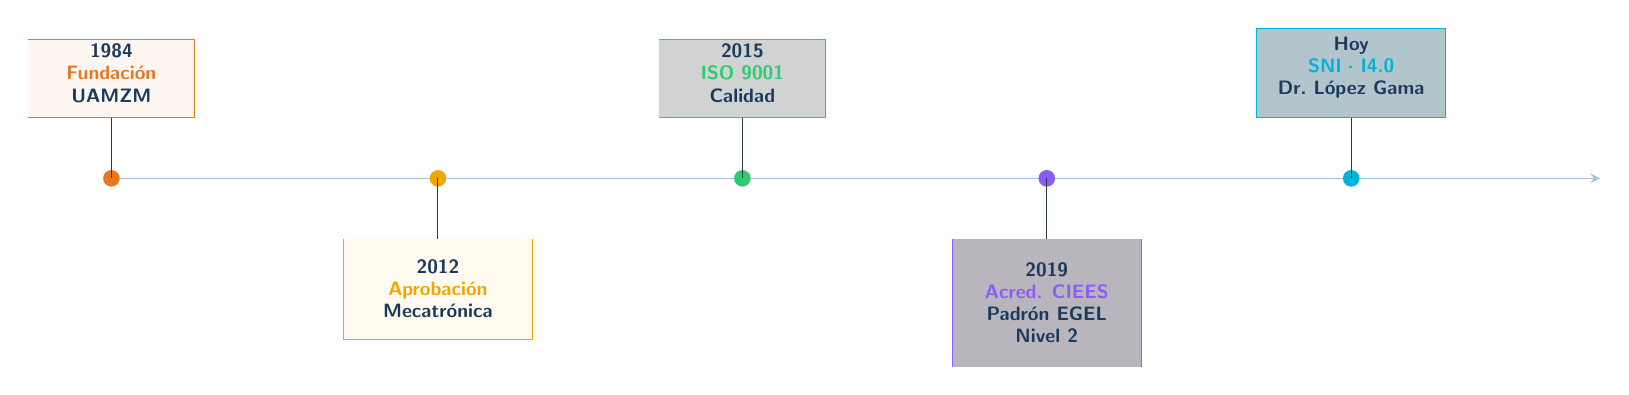
\begin{tikzpicture}[x=1pt, y=1pt,
    every node/.style={font=\fontsize{6.5}{8}\selectfont}]

  \def\LY{0}     % y de la línea central
  \def\XA{0}     % 1984
  \def\XB{118}   % 2012
  \def\XC{228}   % 2015
  \def\XD{338}   % 2019
  \def\XE{448}   % Hoy
  \def\LW{530}   % longitud total

  % ── Línea base ────────────────────────────────────────────
  \draw[lineaAzul, line width=0.6pt]
    (\XA,\LY) -- (\LW,\LY);
  \draw[lineaAzul,->,>=stealth, line width=0.6pt]
    (\LW,\LY) -- (\LW+8,\LY);

  % ── Círculos sobre la línea ───────────────────────────────
  \foreach \x/\col in {
      \XA/naranja, \XB/ambar, \XC/verdeAccento,
      \XD/viola, \XE/cian}{
    \fill[\col] (\x,\LY) circle (3pt);
  }

  % ── 1984 ARRIBA ───────────────────────────────────────────
  \draw[lineaGris, line width=0.4pt]
    (\XA,\LY) -- (\XA,22pt);
  \draw[naranja, line width=0.5pt]
    (\XA-30pt,22pt) rectangle (\XA+30pt,50pt);
  \fill[naranjaClaro!60!blanco]
    (\XA-30pt,22pt) rectangle (\XA+30pt,50pt);
  \node[text=azulOscuro,font=\fontsize{7}{8}\selectfont\bfseries,
        align=center] at (\XA,38pt) {1984\\\textcolor{naranja}{Fundación}\\UAMZM};

  % ── 2012 ABAJO ────────────────────────────────────────────
  \draw[lineaGris, line width=0.4pt]
    (\XB,\LY) -- (\XB,-22pt);
  \draw[ambar, line width=0.5pt]
    (\XB-34pt,-22pt) rectangle (\XB+34pt,-58pt);
  \fill[ambarClaro!60!blanco]
    (\XB-34pt,-22pt) rectangle (\XB+34pt,-58pt);
  \node[text=azulOscuro,font=\fontsize{7}{8}\selectfont\bfseries,
        align=center] at (\XB,-40pt) {2012\\\textcolor{ambar}{Aprobación}\\Mecatrónica};

  % ── 2015 ARRIBA ───────────────────────────────────────────
  \draw[lineaGris, line width=0.4pt]
    (\XC,\LY) -- (\XC,22pt);
  \draw[verdeAccento, line width=0.5pt]
    (\XC-30pt,22pt) rectangle (\XC+30pt,50pt);
  \fill[verdeTech!40!fondoOscuro!20!blanco]
    (\XC-30pt,22pt) rectangle (\XC+30pt,50pt);
  \node[text=azulOscuro,font=\fontsize{7}{8}\selectfont\bfseries,
        align=center] at (\XC,38pt) {2015\\\textcolor{verdeAccento}{ISO 9001}\\Calidad};

  % ── 2019 ABAJO ────────────────────────────────────────────
  \draw[lineaGris, line width=0.4pt]
    (\XD,\LY) -- (\XD,-22pt);
  \draw[viola, line width=0.5pt]
    (\XD-34pt,-22pt) rectangle (\XD+34pt,-68pt);
  \fill[violaFondo!30!blanco]
    (\XD-34pt,-22pt) rectangle (\XD+34pt,-68pt);
  \node[text=azulOscuro,font=\fontsize{7}{8}\selectfont\bfseries,
        align=center] at (\XD,-45pt)
    {2019\\\textcolor{viola}{Acred. CIEES}\\Padrón EGEL\\Nivel 2};

  % ── Hoy ARRIBA ────────────────────────────────────────────
  \draw[lineaGris, line width=0.4pt]
    (\XE,\LY) -- (\XE,22pt);
  \draw[cian, line width=0.5pt]
    (\XE-34pt,22pt) rectangle (\XE+34pt,54pt);
  \fill[cianSuave!30!blanco]
    (\XE-34pt,22pt) rectangle (\XE+34pt,54pt);
  \node[text=azulOscuro,font=\fontsize{7}{8}\selectfont\bfseries,
        align=center] at (\XE,40pt) {Hoy\\\textcolor{cian}{SNI · I4.0}\\Dr.\ López Gama};

\end{tikzpicture}

% ────────────────────────────────────────────────────────────
% PÁG. 4 — TALLERES
% ────────────────────────────────────────────────────────────
\newpage
\BgThispage
\addcontentsline{toc}{section}{Talleres de la Carrera}

\noindent
\tagLabel{verdeAccento}{FORMACIÓN PRÁCTICA}\hspace{4pt}%
\tagLabel{azulOscuro}{TALLERES}

\vspace{6pt}
{\fontsize{20}{24}\selectfont\bfseries\color{azulOscuro}
  TALLERES QUE OFRECE LA CARRERA\par}
\vspace{3pt}
\lineaNaranja
\vspace{2pt}
{\small\color{textoGris}
  Cuatro espacios donde la teor\'ia se convierte en sistemas reales.}
\vspace{6pt}

\begin{multicols}{2}
\begin{cajaTaller}{ELECTRÓNICA}
Primer acercamiento pr\'actico al control de se\~nales.
Resistencias, capacitores, semiconductores, protoboard y PCB.
Osciloscopio y mult\'imetro para diagnosticar comportamientos
el\'ectricos. Forma la base para integrar sensores y actuadores
en semestres posteriores.
\end{cajaTaller}
\vspace{8pt}
\begin{cajaTaller}{MANUFACTURA}
Del dise\~no digital a la pieza f\'isica: torno, fresadora,
impresi\'on 3D y CNC. El estudiante aprende a seleccionar el
proceso de fabricaci\'on adecuado para estructuras duraderas
y funcionales bajo carga operativa real.
\end{cajaTaller}
\columnbreak
\begin{cajaTaller}{PROGRAMACIÓN}
L\'ogica computacional aplicada al control de hardware. C\'odigo
eficiente para microcontroladores en tiempo real: motores,
sensores, comunicaci\'on entre dispositivos. PLCs y plataformas
embebidas estructuran el cerebro de cualquier m\'aquina
mecatr\'onica.
\end{cajaTaller}
\vspace{8pt}
\begin{cajaTaller}{ROBÓTICA}
Convergencia de las tres \'areas anteriores. Ensamble y
calibraci\'on de robots m\'oviles y brazos articulados. Cinem\'atica,
din\'amica, visi\'on artificial y resoluci\'on de problemas en
entornos reales de alto desempe\~no.
\end{cajaTaller}
\end{multicols}

\vspace{6pt}
\fotoRevista[0.60\linewidth]{proyecto_imt2.jpeg}%
  {Materiales y trabajos representativos de los talleres pr\'acticos.}

% ────────────────────────────────────────────────────────────
% PÁG. 5 — HISTORIA + APLICACIONES
% ────────────────────────────────────────────────────────────
\newpage
\BgThispage
\addcontentsline{toc}{section}{Historia y Aplicaciones}

\noindent
\tagLabel{naranja}{CONTEXTO}\hspace{4pt}%
\tagLabel{azulOscuro}{HISTORIA Y APLICACIONES}

\vspace{6pt}
{\fontsize{20}{24}\selectfont\bfseries\color{azulOscuro}
  ORIGEN, EVOLUCIÓN Y CAMPO DE ACCIÓN\par}
\vspace{3pt}
\lineaNaranja\vspace{6pt}

\section{Historia}
\begin{multicols}{2}
\RaggedRight\small\color{textoGris}
El t\'ermino \textit{mecatr\'onica} fue introducido por Tetsuro Mori
en Yaskawa Electric Corporation, Jap\'on, a principios de los 70.
Con la llegada de los microprocesadores e Internet se estableci\'o
primero en aeron\'autica, luego en el sector automotriz y
finalmente en la programaci\'on avanzada.
\columnbreak
\begin{cajaDato}{LÍNEA DEL TIEMPO}
  \itemBullet{\textbf{1969:} T.\ Mori acu\~na el t\'ermino.}
  \itemBullet{\textbf{1970s:} Aeron\'autica y precisi\'on.}
  \itemBullet{\textbf{1980s:} Sector automotriz — ABS.}
  \itemBullet{\textbf{1990s:} Boom de rob\'otica industrial.}
  \itemBullet{\textbf{2000s:} Sistemas embebidos e Internet.}
  \itemBullet{\textbf{2010s–hoy:} I4.0, IoT, IA, gemelos digitales.}
\end{cajaDato}
\end{multicols}

\vspace{4pt}
\fotoRevista[0.5\linewidth]{Proyecto1.jpeg}%
  {Una de las pr\'acticas que puede ejercer un egresado de Mecatr\'onica.}
\vspace{4pt}

\section{Aplicaciones}
\begin{multicols}{2}
\RaggedRight\small\color{textoGris}
La mecatr\'onica act\'ua sobre tres l\'ineas: automatizaci\'on de
procesos, creaci\'on de productos inteligentes e integraci\'on
transversal de electr\'onica y mec\'anica.
\columnbreak
\itemBullet{\textbf{Automotriz:} ABS, tracci\'on, carrocer\'ia.}
\itemBullet{\textbf{Manufactura:} CNC, robots de ensamble.}
\itemBullet{\textbf{Medicina:} pr\'otesis, cirug\'ia rob\'otica.}
\itemBullet{\textbf{Agroindustria:} drones, riego autom\'atico.}
\itemBullet{\textbf{Energ\'ia:} smart grids, turbinas.}
\itemBullet{\textbf{Consumo:} wearables, electrodom\'esticos.}
\end{multicols}
\vspace{4pt}
\begin{citaRevista}
``La mecatr\'onica busca que los productos y proyectos integren
todas las \'areas en un sistema coherente, eficiente y orientado
al usuario.''
\end{citaRevista}

% ════════════════════════════════════════════════════════════
% SECCIÓN 2 — EDITORIAL: EL ADN DEL INGENIERO  (pág. 6)
% ════════════════════════════════════════════════════════════
\clearpage
\newgeometry{margin=0cm}
\pagestyle{empty}
\AddToShipoutPictureBG*{%
  \AtPageLowerLeft{%
    \color{fondoOscuro}\rule{\paperwidth}{\paperheight}}}
\addcontentsline{toc}{section}{Editorial: El ADN del Ingeniero Mecatrónico}

\noindent\vbox to 0pt{%
\begin{tikzpicture}[remember picture,overlay]
  \fill[azulOscuro,opacity=0.6]
    ([xshift=-7cm]current page.north east) --
    (current page.north east) --
    ([yshift=-9cm]current page.north east) -- cycle;
  \fill[naranja]
    (current page.north west) rectangle
    ([yshift=-6pt]current page.north east);
  \fill[naranja]
    (current page.south west) rectangle
    ([yshift=5pt]current page.south east);
  \node[rotate=-45,font=\fontsize{60}{60}\selectfont\bfseries,
        text=azulOscuro,opacity=0.18]
    at ([xshift=-3.5cm,yshift=-3.5cm]current page.north east){EDITORIAL};
\end{tikzpicture}%
\vss}%

\noindent\hspace{0.9cm}%
\begin{minipage}{\dimexpr\paperwidth-1.8cm}
\vspace*{0.75cm}

\noindent
\tagLabel{naranja}{EDITORIAL}\hspace{4pt}%
\tagLabel{azulOscuro}{EDICIÓN ESPECIAL 2026}\hspace{4pt}%
\tagLabel{grisClaro}{ENTREVISTAS}
\vspace{8pt}

{\fontsize{28}{33}\selectfont\bfseries\color{blanco}
  EL ADN DEL\par{\color{naranja}INGENIERO}\par MECATRÓNICO\par}
\vspace{4pt}
\lineaNaranja\vspace{6pt}

\noindent
\begin{minipage}[t]{0.61\linewidth}
\RaggedRight
\noindent
{\fontsize{38}{38}\selectfont\bfseries\color{naranja}L}%
{\small\color{grisTexto}a tecnolog\'ia avanza a un ritmo vertiginoso,
y en el centro de la Cuarta Revoluci\'on Industrial se encuentra
la Ingenier\'ia Mecatr\'onica. Ya no se trata solo de engranajes
o circuitos aislados; se trata de integrar mundos para dar vida
a sistemas inteligentes que resuelven los problemas del ma\~nana.}
\vspace{7pt}

{\small\color{grisTexto}
En esta \textbf{\color{blanco}Edici\'on Especial 2026} salimos de los
laboratorios para adentrarnos en la mente de quienes est\'an
formando a las futuras generaciones de ingenieros.}
\vspace{6pt}

\begin{tcolorbox}[colback=roseFondo,colframe=naranja,
  arc=0pt,boxrule=1.2pt,left=7pt,right=7pt,top=5pt,bottom=5pt]
\centering
{\fontsize{7}{8.5}\selectfont\bfseries\color{naranja}
  PREGUNTA DE ESTA EDICIÓN:}\par\vspace{4pt}
{\small\itshape\color{grisTexto}
  ¿Qu\'e se necesita realmente para sobrevivir y triunfar\par
  en esta carrera? ¿Qu\'e hay detr\'as de las horas de\par
  desvelo, las matem\'aticas aplicadas y los proyectos\par
  que a veces terminan en chispas?}
\end{tcolorbox}
\vspace{6pt}

{\small\color{grisTexto}
A lo largo de estas entrevistas descubrimos que, sin importar la
generaci\'on o especialidad, todos coinciden en un elemento:}
\vspace{6pt}

\begin{tcolorbox}[colback=fondoOscuro,colframe=naranja,
  arc=0pt,boxrule=0pt,left=0pt,right=0pt,top=0pt,bottom=0pt]
\noindent{\color{lineaGris}\rule{\linewidth}{0.4pt}}\par\vspace{4pt}
\centering
{\fontsize{22}{26}\selectfont\bfseries\color{naranja}
  LA\ \ CURIOSIDAD.}
\par\vspace{4pt}
\noindent{\color{lineaGris}\rule{\linewidth}{0.4pt}}
\end{tcolorbox}
\vspace{6pt}

{\small\color{grisTexto}
Si eres un estudiante buscando inspiraci\'on para tu pr\'oximo
proyecto, o un aspirante pregunt\'andote si debes temerle a las
matem\'aticas, \textbf{\color{blanco}esta edici\'on est\'a
dise\~nada para ti}.}
\vspace{8pt}

\begin{tcolorbox}[colback=azulOscuro,colframe=naranja,
  arc=0pt,boxrule=1pt,left=8pt,right=8pt,top=6pt,bottom=6pt]
\small\color{grisTexto}
\textbf{\color{blanco}Bienvenidos a la ingenier\'ia que conecta mundos.}\par
\textbf{\color{naranja}Bienvenidos a Mecatr\'onica.}
\end{tcolorbox}
\end{minipage}%
\hfill
\begin{minipage}[t]{0.35\linewidth}
\vspace{0pt}
{\fontsize{7}{8.5}\selectfont\bfseries\color{naranja}
  EN ESTA EDICIÓN ENTREVISTAMOS A:}\par
\vspace{2pt}
{\color{naranja}\rule{\linewidth}{0.8pt}}\par\vspace{6pt}

\tarjetaPersona{ambar}%
  {Ing. Víctor Esteban Espinosa López}%
  {Docente TC · Fundador de la carrera · UASLP}{7}
\tarjetaPersona{cian}%
  {Dr. Roberto C. Martínez Montejano}%
  {Prof. Investigador TC · SNI · Secretario Planeación}{8}
\tarjetaPersona{viola}%
  {Dr. Germánico González Badillo}%
  {Secretario Escolar · Prof. Investigador TC}{9}
\tarjetaPersona{naranja}%
  {Benny Martínez}%
  {Estudiante 6° sem. · Drones NIR · Automatización}{10}
\tarjetaPersona{verdeAccento}%
  {Gael}%
  {Estudiante 6° sem. · Control PID · Industria 4.0}{11}
\tarjetaPersona{verdeAccento}%
  {Erick Moreno Negrete}%
  {Estudiante · Ingeniería Mecatrónica · UASLP}{15}
\tarjetaPersona{rose}%
  {Mtra. Ivana López Reina}%
  {Docente · Campus Río Verde · UASLP}{16}

\vspace{6pt}
{\color{lineaGris}\rule{\linewidth}{0.4pt}}\par\vspace{5pt}
{\fontsize{6.5}{8.5}\selectfont\color{lineaAzul}
  \textit{Entrevistas realizadas en la Facultad de Ingenier\'ia
  de la UASLP, primer trimestre 2026.}}
\end{minipage}

\pieRevista{naranja}{6}
\vspace*{0.45cm}
\end{minipage}

\clearpage
\restoregeometry
\pagestyle{fancy}

% ════════════════════════════════════════════════════════════
% PÁG. 7 — ENTREVISTA DR. VÍCTOR ESPINOSA (barra vertical)
% ════════════════════════════════════════════════════════════
\clearpage
\newgeometry{margin=0cm}
\pagestyle{empty}
\AddToShipoutPictureBG*{%
  \AtPageLowerLeft{%
    \color{fondoOscuro}\rule{\paperwidth}{\paperheight}}}
\addcontentsline{toc}{section}{Entrevista: Ing. Víctor Esteban Espinosa}

% TikZ overlay sin espacio vertical — envuelto en vbox de altura 0
\noindent\vbox to 0pt{%
\begin{tikzpicture}[remember picture,overlay]
  \fill[azulOscuro]
    (current page.north west) rectangle
    ([xshift=3.8cm]current page.south west);
  \fill[ambar]
    ([xshift=3.8cm]current page.north west) rectangle
    ([xshift=4.05cm]current page.south west);
  \draw[naranja,line width=5pt]
    (current page.north west) -- (current page.north east);
  \node[rotate=90,anchor=center,
        font=\fontsize{7}{8}\selectfont\bfseries,
        text=ambar,opacity=0.35]
    at ([xshift=1.9cm,yshift=0cm]current page.west)
    {D\ \ O\ \ C\ \ E\ \ N\ \ T\ \ E\ \ \ \ \ E\ \ N\ \ T\ \ R\ \ E\ \ V\ \ I\ \ S\ \ T\ \ A};
  % Foto Víctor — colocar en victor.jpg
  \draw[ambar,line width=1.2pt]
    ([xshift=0.4cm,yshift=-1.8cm]current page.north west) rectangle
    ([xshift=3.4cm,yshift=-5.4cm]current page.north west);
  \node[inner sep=0pt] at ([xshift=1.9cm,yshift=-3.6cm]current page.north west)
    {\IfFileExists{Entrevista_DrVictor.jpeg}{%
       \includegraphics[width=4.0cm,height=4.6cm,keepaspectratio]{Entrevista_DrVictor.jpeg}%
     }{%
       \textcolor{blanco}{\fontsize{6.5}{8}\selectfont\bfseries FOTO}%
     }};
  \node[anchor=north,font=\fontsize{8}{10}\selectfont\bfseries,
        text=blanco,align=center,text width=3.0cm]
    at ([xshift=1.9cm,yshift=-5.6cm]current page.north west)
    {V\'ICTOR E.\\ ESPINOSA L.};
  \draw[ambar,line width=0.8pt]
    ([xshift=0.4cm,yshift=-6.6cm]current page.north west) --
    ([xshift=3.4cm,yshift=-6.6cm]current page.north west);
  \node[anchor=north west,text width=3.0cm,
        font=\fontsize{6.5}{8.5}\selectfont,
        text=grisTexto,align=left]
    at ([xshift=0.42cm,yshift=-6.9cm]current page.north west)
    {\textcolor{ambar}{\bfseries CARGO}\par
     Docente tiempo completo\par\vspace{3pt}
     \textcolor{ambar}{\bfseries FORMACIÓN}\par
     Ing.\ Electrónico · M.C.\ y Dr.\ (c) en Ing.\ Eléctrica\par\vspace{3pt}
     \textcolor{ambar}{\bfseries INSTITUCIÓN}\par UASLP\par\vspace{3pt}
     \textcolor{ambar}{\bfseries TRAYECTORIA}\par
     Fundador de la carrera en campus foráneo, 2012\par\vspace{3pt}
     \textcolor{ambar}{\bfseries EXPERIENCIA}\par
     $\sim$14 años formando ingenieros\par\vspace{3pt}
     \textcolor{ambar}{\bfseries VISIÓN}\par
     El mecatrónico: traductor y líder multidisciplinario};
  \draw[ambar,line width=0.6pt,opacity=0.4]
    ([xshift=0.4cm,yshift=1.5cm]current page.south west) --
    ([xshift=3.4cm,yshift=1.5cm]current page.south west);
  \node[font=\fontsize{6}{7}\selectfont\bfseries,
        text=ambar,opacity=0.6,align=center]
    at ([xshift=1.9cm,yshift=0.9cm]current page.south west){MARZO 2026};
\end{tikzpicture}%
\vss}%

\noindent\hspace{4.4cm}%
\begin{minipage}{\dimexpr\paperwidth-5.2cm}
\vspace*{0.55cm}

\tagLabel{ambar}{ENTREVISTA DOCENTE}\hspace{4pt}%
\tagLabel{azulOscuro}{FUNDADORES DE CARRERA}
\vspace{6pt}

{\fontsize{22}{26}\selectfont\bfseries\color{blanco}
  CURIOSO Y VALIENTE:\par{\color{ambar}14 AÑOS} FORMANDO INGENIEROS\par}
\vspace{3pt}
\lineaAmbar\vspace{2pt}
{\small\color{grisTexto}
  El Mtro.\ V\'ictor Esteban Espinosa L\'opez, fundador de la carrera
  en su campus, comparte su visi\'on sobre el perfil del mecatr\'onico.}
\vspace{7pt}

\begin{multicols}{2}\RaggedRight

\preguntaA{¿Qu\'e se necesita para ser maestro de Mecatr\'onica?}
\respuestaS{Principalmente una licenciatura y el gusto por compartir
conocimientos. Para la parte disciplinar s\'i se requiere experiencia
t\'ecnica y afinidad.}

\preguntaA{¿Qu\'e caracteriza a los alumnos de Mecatr\'onica?}
\respuestaS{La curiosidad y las ganas de aprender c\'omo funcionan
los aparatos electr\'onicos. Generaciones muy proactivas, respetuosas
y con inter\'es genuino por investigar.}

\preguntaA{¿Cu\'al es el factor clave para su \'exito?}
\respuestaS{Esa misma curiosidad. Cuando un alumno quiere saber
c\'omo funcionan las cosas, \'el mismo se da cuenta de que necesita
aprender y practicar por su cuenta.}

\preguntaA{¿Qu\'e tan dif\'icil es darles clase?}
\respuestaS{Es muy f\'acil. Como tienen tantas ganas de aprender
y son muy respetuosos, dirigir una clase con ellos es gratificante.}

\preguntaA{¿Qu\'e mensaje transmite a los futuros ingenieros?}
\respuestaS{Que ``s\'i se puede''. Yo mismo soy electr\'onico y tuve
que aprender mec\'anica sobre la marcha. Con tiempo y preparaci\'on,
cualquier deficiencia se supera.}

\columnbreak

\preguntaA{¿Qu\'e disfruta m\'as de la Mecatr\'onica?}
\respuestaS{El razonamiento te\'orico, porque da las bases para
resolver problemas. Y la parte pr\'actica, donde los alumnos
se acercan a proyectos reales.}

\preguntaA{¿Le habr\'ia gustado estudiar Mecatr\'onica?}
\respuestaS{S\'i, me habr\'ia encantado. Me habr\'ia gustado conocer
a fondo la mec\'anica, la rob\'otica y la automatizaci\'on desde
mi formaci\'on inicial.}

\preguntaA{¿Qu\'e le dir\'ia a un aspirante que duda?}
\respuestaS{Que no se preocupe por el nivel de conocimientos al
inicio. Que tenga curiosidad y ganas de investigar c\'omo funcionan
las m\'aquinas. Eso vale m\'as.}

\preguntaA{¿Qu\'e aporta el mecatr\'onico a la industria?}
\respuestaS{Son el enlace. Traductores entre especialistas que
hablan ``idiomas'' distintos, con capacidad de liderazgo para
unir las partes y hacer avanzar los proyectos.}

\vspace{6pt}
\begin{tcolorbox}[colback=ambarFondo,colframe=ambar,
  arc=0pt,boxrule=1.2pt,left=6pt,right=6pt,top=5pt,bottom=5pt]
\centering\fontsize{7}{8}\selectfont\bfseries\color{ambar}
EN UNA FRASE:\par\vspace{3pt}
\itshape\footnotesize\color{blanco}
``Un ingeniero mecatr\'onico\\ es curioso y valiente.''
\end{tcolorbox}
\end{multicols}
\vspace*{11.30cm}

\pieRevista{ambar}{7}
\vspace*{0.45cm}
\end{minipage}

\clearpage
\restoregeometry
\pagestyle{fancy}

% ════════════════════════════════════════════════════════════
% PÁGS. 8–9 — ENTREVISTA DR. MARTÍNEZ MONTEJANO
% ════════════════════════════════════════════════════════════
\clearpage
\newgeometry{margin=0cm}
\pagestyle{empty}
\AddToShipoutPictureBG*{%
  \AtPageLowerLeft{%
    \color{fondoOscuro}\rule{\paperwidth}{\paperheight}}}
\addcontentsline{toc}{section}{Entrevista: Dr. Roberto C. Martínez Montejano}

\noindent\vbox to 0pt{%
\begin{tikzpicture}[remember picture,overlay]
  \fill[cianSuave]
    (current page.north west) rectangle
    ([yshift=-4.6cm]current page.north east);
  \fill[cian]
    ([yshift=-4.6cm]current page.north west) rectangle
    ([yshift=-4.85cm]current page.north east);
  \fill[naranja]
    (current page.north west) rectangle
    ([yshift=-5pt]current page.north east);
  \draw[cian,line width=1.2pt]
    ([xshift=0.8cm,yshift=-0.5cm]current page.north west) rectangle
    ([xshift=3.6cm,yshift=-4.1cm]current page.north west);
  \node[inner sep=0pt] at ([xshift=2.2cm,yshift=-2.3cm]current page.north west)
    {\IfFileExists{Entrevista_DrRoberto.jpeg}{%
       \includegraphics[width=3.6cm,height=4.4cm,keepaspectratio]{Entrevista_DrRoberto.jpeg}%
     }{%
       \textcolor{blanco}{\fontsize{7}{8}\selectfont\bfseries FOTO}%
     }};
  \node[anchor=north west,font=\fontsize{16}{19}\selectfont\bfseries,text=blanco]
    at ([xshift=4.1cm,yshift=-0.55cm]current page.north west)
    {DR. ROBERTO C.};
  \node[anchor=north west,font=\fontsize{16}{19}\selectfont\bfseries,text=cian]
    at ([xshift=4.1cm,yshift=-1.35cm]current page.north west)
    {MARTÍNEZ MONTEJANO};
  \draw[cian,line width=0.7pt]
    ([xshift=4.1cm,yshift=-2.05cm]current page.north west) --
    ([xshift=17.5cm,yshift=-2.05cm]current page.north west);
  \node[anchor=north west,text width=6.0cm,
        font=\fontsize{7}{9}\selectfont,text=grisTexto]
    at ([xshift=4.1cm,yshift=-2.25cm]current page.north west)
    {\textcolor{cian}{\bfseries CARGO}\par
     Prof. Investigador TC · Mecatrónica\par
     Secretario de Planeación\par\smallskip
     \textcolor{cian}{\bfseries FORMACIÓN}\par
     Ing.\ Electrónico · M.C.\ y Dr.\ en Ciencias Aplicadas};
  \node[anchor=north west,text width=6.0cm,
        font=\fontsize{7}{9}\selectfont,text=grisTexto]
    at ([xshift=10.5cm,yshift=-2.25cm]current page.north west)
    {\textcolor{cian}{\bfseries ESPECIALIZACIÓN}\par
     Control no lineal · Electrónica de potencia\par
     Instrumentación · Robótica\par\smallskip
     \textcolor{cian}{\bfseries RECONOCIMIENTO}\par
     Sistema Nacional de Investigadores (SNI)};
  \node[anchor=south east]
    at ([xshift=-0.5cm,yshift=-4.25cm]current page.north east)
    {\tagLabel{naranja}{INVESTIGADOR SNI}\hspace{3pt}%
     \tagLabel{azulOscuro}{UASLP · 2013--HOY}};
\end{tikzpicture}%
\vss}%

\vspace*{5.2cm}
\noindent\hspace{0.85cm}%
\begin{minipage}{\dimexpr\paperwidth-1.7cm}

{\fontsize{12}{15}\selectfont\bfseries\color{blanco}
  VERSATILIDAD, RIGOR Y COMUNIDAD:\par
  {\color{cian}LA MECATRÓNICA VISTA DESDE LA INVESTIGACIÓN}\par}
\vspace{2pt}\lineaCian\vspace{1pt}
{\small\color{grisTexto}
  M\'as de una d\'ecada en el aula, coordinaci\'on de carrera y
  proyectos publicables a nivel internacional.}
\vspace{5pt}

\resetQ
\begin{bloqueQ}{cian}{Bloque I · Visión Académica y Docencia}
\begin{multicols}{2}\RaggedRight
\preguntaC{¿Qu\'e necesita para ser maestro de Mecatr\'onica?}
\respuestaS{Entender los conocimientos a la perfecci\'on. Cuando
haces tuyo el conocimiento es m\'as f\'acil explic\'arselo a
alguien que parte de cero. Hay que recordar que fuiste estudiante.}
\preguntaC{¿Hace cu\'anto da clases?}
\respuestaS{Empec\'e en 2013 durante el doctorado: Tecmilenio y
Tec de Monterrey. En 2016 entr\'e a UASLP; en 2017 gan\'e la
plaza de profesor investigador TC.}
\preguntaC{¿Qu\'e caracteriza a un alumno de Mecatr\'onica?}
\respuestaS{La versatilidad. Una sola persona domina rob\'otica,
dise\~no CAD e impresi\'on 3D. El mecatr\'onico se est\'a comiendo
el campo laboral del ingeniero en electr\'onica.}
\preguntaC{¿Factores para sobrellevar la carrera?}
\respuestaS{Manejo del tiempo, del estr\'es y trabajo en equipo.
Con hasta 10 materias es imposible sobrevivir solo.}
\columnbreak
\preguntaC{¿Qu\'e tan dif\'icil es ser su maestro?}
\respuestaS{No mucho. Empec\'e a los 23 a\~nos. Siempre quise
ser el profesor que yo hubiera querido tener.}
\preguntaC{¿Qu\'e transmite m\'as all\'a del temario?}
\respuestaS{El conocimiento puro. Me enorgullece que digan:
``podr\'a caerte bien o mal, pero siempre aprendes algo''.}
\preguntaC{¿Qu\'e m\'as le gusta de la Mecatr\'onica?}
\respuestaS{Como maestro, los proyectos que alcanzan niveles
publicables internacionalmente. Eso me mantiene en el SNI.}
\preguntaC{¿Le hubiera gustado estudiar Mecatr\'onica?}
\respuestaS{Obviamente. Cuando entr\'e a Electr\'onica en 2006,
Mecatr\'onica abri\'o en SLP hasta 2007.}
\preguntaC{¿Qu\'e le dir\'ia a quien quiere ingresar?}
\respuestaS{Que no le tengan miedo a las matem\'aticas: son muchas
pero aplicadas. Con ganas de aprender, ya est\'an del otro lado.}
\end{multicols}
\end{bloqueQ}
\vspace*{10.30cm}

\pieRevista{cian}{8}
\vspace*{0.25cm}
\end{minipage}

% ── Página 9 — Bloque coordinación ──────────────────────────
\newpage
\AddToShipoutPictureBG*{%
  \AtPageLowerLeft{%
    \color{fondoOscuro}\rule{\paperwidth}{\paperheight}}}

\noindent\vbox to 0pt{%
\begin{tikzpicture}[remember picture,overlay]
  \fill[naranja](current page.north west) rectangle
    ([yshift=-5pt]current page.north east);
  \fill[cianSuave]([yshift=-5pt]current page.north west) rectangle
    ([yshift=-1.1cm]current page.north east);
  \node[anchor=west,font=\fontsize{9}{11}\selectfont\bfseries,text=cian]
    at ([xshift=0.9cm,yshift=-0.55cm]current page.north west)
    {DR. ROBERTO C. MARTÍNEZ MONTEJANO};
  \node[anchor=east,font=\fontsize{7}{8}\selectfont,text=grisTexto]
    at ([xshift=-0.9cm,yshift=-0.55cm]current page.north east)
    {COORDINACIÓN · INVESTIGACIÓN · DOCENCIA};
\end{tikzpicture}%
\vss}%

\vspace*{1.4cm}
\noindent\hspace{0.85cm}%
\begin{minipage}{\dimexpr\paperwidth-1.7cm}

\resetQ
\begin{bloqueQ}{naranja}{Bloque II · Experiencia como Coordinador de Carrera}
\begin{multicols}{2}\RaggedRight
\preguntaC{¿Cu\'ales son las funciones del coordinador?}
\respuestaS{Eres el intermediario entre alumnos, profesores y
autoridades. Planeas horarios, gestionas tutor\'ias y garantizas
que la carrera avance. Estamos en el padr\'on de excelencia del
EGEL. Much\'isima chamba —sin remuneraci\'on extra.}
\preguntaC{¿Qu\'e fue lo que m\'as disfrut\'o?}
\respuestaS{Hablar con los alumnos y solucionar sus problemas.
Me ten\'ian confianza y busc\'abamos resolverlas juntos.}
\columnbreak
\preguntaC{¿Cu\'al fue su reto m\'as dif\'icil?}
\respuestaS{Lograr la acreditaci\'on del EGEL y consolidar los
``Retos Buchidos'' con el Dr.\ Jimmy: primeros y terceros lugares,
incluyendo el 1er lugar en 2023 con el equipo de Rams\'es.}
\preguntaC{¿Qu\'e consejo le dar\'ia al nuevo coordinador?}
\respuestaS{Mucha paciencia y organizar su tiempo. Cada d\'ia
pasa algo inesperado: siempre hay algo que resolver.}
\end{multicols}
\end{bloqueQ}
\vspace{3pt}

\noindent
\begin{minipage}[t]{0.44\linewidth}
\vspace{0pt}
\begin{citaCian}
``No le tengan miedo a las matem\'aticas.
Son muchas, pero son aplicadas. Con ganas
de aprender, ya est\'an del otro lado.''
\end{citaCian}
\vspace{5pt}
\begin{tcolorbox}[colback=cianSuave,colframe=cian,
  arc=0pt,boxrule=0.8pt,left=6pt,right=6pt,top=5pt,bottom=5pt]
{\fontsize{7.5}{9}\selectfont\bfseries\color{cian}
  TRAYECTORIA EN CIFRAS}\par
\vspace{2pt}{\color{cian}\rule{\linewidth}{0.4pt}}\par\vspace{3pt}
\renewcommand{\arraystretch}{1.3}
\begin{tabular}{@{}r@{\hspace{6pt}}l@{}}
  \textcolor{cian}{\textbf{2013}} & \footnotesize\color{grisTexto}Inicio docente\\
  \textcolor{cian}{\textbf{2016}} & \footnotesize\color{grisTexto}Ingresa a UASLP\\
  \textcolor{cian}{\textbf{2017}} & \footnotesize\color{grisTexto}Plaza TC Investigador\\
  \textcolor{cian}{\textbf{2023}} & \footnotesize\color{grisTexto}1\textordmasculine\ lugar Retos Buchidos\\
  \textcolor{cian}{\textbf{Hoy}}  & \footnotesize\color{grisTexto}SNI · Secretario Planeación\\
\end{tabular}
\end{tcolorbox}
\end{minipage}%
\hfill
\begin{minipage}[t]{0.52\linewidth}
\vspace{0pt}
\begin{tcolorbox}[colback=cianSuave,colframe=naranja,
  arc=0pt,boxrule=0.8pt,left=7pt,right=7pt,top=5pt,bottom=5pt]
{\fontsize{7.5}{9}\selectfont\bfseries\color{naranja}
  CLAVES SEGÚN EL DR. MARTÍNEZ}\par
\vspace{2pt}{\color{naranja}\rule{\linewidth}{0.4pt}}\par\vspace{3pt}
\itemC{\textbf{Buen maestro:} hacer tuyo el conocimiento.}
\itemC{\textbf{Sobrevivir la carrera:} tiempo, estr\'es, comunidad.}
\itemC{\textbf{Entrar a Mecatr\'onica:} curiosidad aplicada.}
\itemC{\textbf{Coordinar:} paciencia infinita y agenda blindada.}
\itemC{\textbf{El mecatr\'onico:} el traductor que une todos.}
\end{tcolorbox}
\end{minipage}
\vspace*{13.30cm}

\pieRevista{cian}{9}
\vspace*{0.35cm}
\end{minipage}

\clearpage
\restoregeometry
\pagestyle{fancy}

% ════════════════════════════════════════════════════════════
% PÁG. 10 — ENTREVISTA DR. GERMÁNICO GONZÁLEZ (grid violeta)
% ════════════════════════════════════════════════════════════
\clearpage
\newgeometry{margin=0cm}
\pagestyle{empty}
\AddToShipoutPictureBG*{%
  \AtPageLowerLeft{%
    \color{fondoOscuro}\rule{\paperwidth}{\paperheight}}}
\addcontentsline{toc}{section}{Entrevista: Dr. Germánico González Badillo}

\noindent\vbox to 0pt{%
\begin{tikzpicture}[remember picture,overlay]
  \fill[violaOscuro]
    (current page.north west) --
    ([xshift=8.5cm]current page.north west) --
    ([yshift=-4.5cm]current page.north west) -- cycle;
  \draw[viola,line width=1.5pt]
    ([xshift=8.5cm]current page.north west) --
    ([yshift=-4.5cm]current page.north west);
  \fill[naranja]
    (current page.north west) rectangle
    ([yshift=-5pt]current page.north east);
  \fill[naranja]
    (current page.south west) rectangle
    ([yshift=4pt]current page.south east);
  \foreach \x in {0,0.35,...,3.5}{
    \foreach \y in {0,0.35,...,2.5}{
      \fill[viola,opacity=0.15]
        ([xshift=-\x cm-0.5cm,yshift=\y cm+0.4cm]current page.south east)
        circle (1.2pt);}}
  \draw[violaMedio,line width=18pt,opacity=0.25]
    ([xshift=-3.2cm,yshift=-5.5cm]current page.north east) circle (3.8cm);
  \node[font=\fontsize{120}{120}\selectfont\bfseries,
        text=violaMedio,opacity=0.12]
    at ([xshift=-2.5cm,yshift=-5.0cm]current page.north east){13};
\end{tikzpicture}%
\vss}%

\noindent\hspace{0.85cm}%
\begin{minipage}{\dimexpr\paperwidth-1.7cm}
\vspace*{0.45cm}

\noindent
\begin{minipage}[t]{0.57\linewidth}
\vspace{0pt}
\tagLabel{viola}{ENTREVISTA DOCENTE}\hspace{4pt}%
\tagLabel{azulOscuro}{13 AÑOS · UASLP}
\vspace{7pt}

{\fontsize{10}{13}\selectfont\bfseries\color{viola}
  SECRETARIO ESCOLAR · PROFESOR INVESTIGADOR}\par
\vspace{2pt}
{\fontsize{24}{28}\selectfont\bfseries\color{blanco}
  DEDICADO:\par{\color{viola}EL PUENTE} QUE\par CONECTA MUNDOS\par}
\vspace{3pt}
\lineaViola\vspace{3pt}
{\small\color{grisTexto}
  El Dr.\ Germ\'anico Gonz\'alez lleva 13 a\~nos demostrando
  que la mecatr\'onica no es solo industria: es emprendimiento
  y, sobre todo, dedicaci\'on.}
\end{minipage}%
\hfill
\begin{minipage}[t]{0.39\linewidth}
\vspace{0pt}
\begin{tcolorbox}[colback=violaMedio,colframe=viola,
  arc=0pt,boxrule=1pt,left=7pt,right=7pt,top=6pt,bottom=6pt]

\begin{tikzpicture}
  \fill[violaOscuro] (0,0) rectangle (4.5cm,2.0cm);
  \draw[viola,line width=1pt] (0,0) rectangle (4.5cm,2.0cm);
  \node[inner sep=0pt] at (2.25cm,1.0cm)
    {\IfFileExists{Entrevista_DrGermanico.jpeg}{%
       \includegraphics[width=6.5cm,height=4.0cm,keepaspectratio]{Entrevista_DrGermanico.jpeg}%
     }{%
       \textcolor{grisTexto}{\fontsize{7}{8}\selectfont\bfseries FOTO}%
     }};
\end{tikzpicture}\par\vspace{4pt}
{\fontsize{8.5}{10}\selectfont\bfseries\color{blanco}
  DR. GERMÁNICO\par GONZÁLEZ BADILLO}\par
\vspace{2pt}{\color{viola}\rule{\linewidth}{0.5pt}}\par\vspace{3pt}
\itemPerfil{Cargo}{Secretario Escolar · Prof.\ Investigador TC}
\itemPerfil{Formación}{Ing.\ Mec.\ Adm.\ · M.C.\ Automotriz\par
  Dr.\ Ing.\ Mecánica (mecatrónicos)}
\itemPerfil{Exp.\ + Visión}{13 años · Industria y emprendimiento}
\end{tcolorbox}
\end{minipage}

\vspace{4pt}
\lineaGrisH\vspace{3pt}

\begin{multicols}{3}
\tarjetaQA{viola}{¿Qué se necesita para ser maestro?}%
  {Dos perfiles: hora clase (grado + experiencia pr\'actica)
  y tiempo completo (convocatoria + Doctorado en Ingenier\'ia).}
\tarjetaQA{naranja}{¿Qué caracteriza a un alumno?}%
  {Son curiosos, disfrutan armar y desarmar. Los percibo m\'as
  responsables que quienes eligen carreras menos exigentes.}
\tarjetaQA{viola}{¿Factor principal del éxito?}%
  {La dedicaci\'on. En 13 a\~nos los que triunfan son los que
  se concentran, estudian y construyen buenas relaciones.}
\columnbreak
\tarjetaQA{naranja}{¿Qué tan difícil es ser su maestro?}%
  {F\'acil. Por su sed de aprender, encargas un proyecto y
  la mayor\'ia busca el conocimiento por cuenta propia.}
\tarjetaQA{viola}{¿Qué transmite más allá del temario?}%
  {La seguridad. Que conf\'ien en s\'i mismos y en lo que son
  capaces de hacer con los conocimientos que adquieren.}
\tarjetaQA{naranja}{¿Le habría gustado estudiar Mecatrónica?}%
  {Definitivamente. Cuando estudi\'e no exist\'ia en M\'exico.
  La electr\'onica tuve que aprenderla de forma autodidacta.}
\columnbreak
\tarjetaQA{viola}{¿Qué más disfruta como maestro?}%
  {Ver crecer a mis alumnos: desde los primeros semestres
  hasta el examen profesional. Ese cambio me llena.}
\tarjetaQA{naranja}{¿Cómo contribuye el mecatrónico?}%
  {Sirve de puente. No reemplaza especialistas, pero los
  enlaza para avanzar el desarrollo tecnol\'ogico.}
\tarjetaQA{viola}{¿Qué le diría a un aspirante de prepa?}%
  {Que se decida: es una de las carreras mejor pagadas. Solo
  necesita gusto genuino por saber c\'omo funcionan las cosas.}
\end{multicols}

\vspace{3pt}
\noindent
\begin{minipage}[t]{0.48\linewidth}
\vspace{0pt}
\begin{tcolorbox}[colback=violaFondo,colframe=viola,
  arc=0pt,boxrule=1pt,left=7pt,right=7pt,top=6pt,bottom=6pt]
{\fontsize{7.5}{9}\selectfont\bfseries\color{viola}
  ¿QUÉ LO HACE ÚNICO?}\par
\vspace{2pt}{\color{viola}\rule{\linewidth}{0.4pt}}\par\vspace{4pt}
{\footnotesize\color{grisTexto}
  Es una carrera de mucha aplicaci\'on. El mecatr\'onico puede
  \textbf{\color{viola}emprender, poner su propio taller o
  f\'abrica}. Tiene muchas ramas de utilidad hoy en d\'ia.}
\end{tcolorbox}
\end{minipage}%
\hfill
\begin{minipage}[t]{0.48\linewidth}
\vspace{0pt}
\begin{tcolorbox}[colback=violaMedio,colframe=naranja,
  arc=0pt,boxrule=1.2pt,left=8pt,right=8pt,top=8pt,bottom=8pt]
\centering
{\fontsize{7}{8.5}\selectfont\bfseries\color{naranja}EN UNA FRASE:}\par
\vspace{5pt}
{\fontsize{13}{16}\selectfont\bfseries\color{blanco}
  ``Un ingeniero\par mecatr\'onico\par}
{\fontsize{13}{16}\selectfont\bfseries\color{viola}es dedicado.''\par}
\vspace{3pt}
{\fontsize{7}{8}\selectfont\color{grisTexto}— Dr.\ Germ\'anico Gonz\'alez}
\end{tcolorbox}
\end{minipage}

\pieRevista{viola}{10}
\vspace*{0.38cm}
\end{minipage}

\clearpage
\restoregeometry
\pagestyle{fancy}

% ════════════════════════════════════════════════════════════
% PÁG. 11 — ENTREVISTA BENNY
% ════════════════════════════════════════════════════════════
\clearpage
\newgeometry{margin=0cm}
\pagestyle{empty}
\AddToShipoutPictureBG*{%
  \AtPageLowerLeft{%
    \color{fondoOscuro}\rule{\paperwidth}{\paperheight}}}
\addcontentsline{toc}{section}{Entrevista: Benny Martínez (Estudiante)}

\noindent\hspace{1.0cm}%
\begin{minipage}{\dimexpr\paperwidth-2.0cm}
\vspace*{0.50cm}

\barraAccento
\noindent
\begin{minipage}[t]{0.55\linewidth}
  {\fontsize{26}{30}\selectfont\bfseries\color{blanco}
    ENTREVISTA:\\ENTRE DRONES,\\CULTIVOS Y PLC\par}
  \vspace{5pt}\lineaNaranja
  {\small\color{grisTexto}
    Un estudiante nos habla de sus retos acad\'emicos,
    su proyecto de detecci\'on de estr\'es en plantas con drones
    y su sue\~no de trabajar en BMW.}
\end{minipage}%
\hfill
\begin{minipage}[t]{0.40\linewidth}
  \vspace{0pt}\centering
  \fotoPersona{Entrevista_Benito.jpeg}{5.4cm}{4.8cm}\\[4pt]
  \colorbox{azulOscuro}{\parbox{4.4cm}{\centering
    \textcolor{blanco}{\footnotesize\bfseries
      BENNY\\ESTUDIANTE DE MECATR\'ONICA}}}
\end{minipage}

\vspace{7pt}\lineaGrisH\vspace{5pt}

\begin{multicols}{3}
\footnotesize\color{grisTexto}\RaggedRight

Mecatr\'onica suena a robots gigantes, pero quienes la viven saben que
es mucho m\'as: control, manufactura, programaci\'on y trabajo en equipo.
Benny cursa esta carrera y nos cuenta su experiencia sin filtros.

\preguntaN{¿Qu\'e ha sido lo m\'as pesado hasta ahora?}
\respuestaS{Control 1 y 2. Es el filtro m\'as grande de toda la carrera;
ah\'i se quedan la mayor\'ia de los alumnos.}

\preguntaN{¿Cu\'ando entendiste c\'omo se conecta todo?}
\respuestaS{En sexto semestre, en dise\~no mecatr\'onico. Ah\'i aplicas
todo lo aprendido desarrollando tu propio proyecto.}

\columnbreak

\preguntaN{¿Qu\'e \'area te ha sorprendido m\'as?}
\respuestaS{Manufactura. C\'odigos G y alto costo de error en la CNC
— esa m\'aquina vale millones.}

\vspace{4pt}
\begin{citaDestacada}
``Escoge algo que te llame la atenci\'on, porque si no se te
har\'a muy pesado y frustrante.''
\end{citaDestacada}

\preguntaN{¿Qu\'e habilidad necesitas desarrollar m\'as?}
\respuestaS{La comunicaci\'on. La escuela no nos la da; es la
asignatura pendiente de la ingenier\'ia.}

\columnbreak

\preguntaN{¿Qu\'e consejo te dar\'ias al comenzar?}
\respuestaS{Que hubiera pensado mejor las cosas. La carrera es
muy pesada y lleva mucho tiempo.}

\preguntaN{¿C\'omo te organizas para no colapsar?}
\respuestaS{Levant\'andome a las 5 de la ma\~nana todos los d\'ias.}

\vspace{5pt}
Su meta: BMW, \'area de automatizaci\'on con PLC — la disciplina
que m\'as le apasiona dentro de la carrera.
\end{multicols}

\vspace{5pt}\lineaGrisH\vspace{7pt}

\noindent
\begin{minipage}[]{0.62\linewidth}
{\small\bfseries\color{blanco}EL PROYECTO: DRONES PARA DETECTAR ESTR\'ES EN PLANTAS}\par
\vspace{4pt}
\begin{multicols}{2}\footnotesize\color{grisTexto}\RaggedRight
Drone Phantom 4 Pro con filtro NIR sobrevuela cultivos. Un algoritmo
de IA compara las im\'agenes con una referencia sana y genera alertas
preventivas para evitar p\'erdidas del cultivo.
\columnbreak
\preguntaN{¿Qu\'e tecnolog\'ias integra?}
\respuestaS{Drone, c\'amara NIR, Pix4D para rutas y MATLAB para datos.
El algoritmo de IA ya est\'a desarrollado.}
\preguntaN{¿Qu\'e conocimientos aplicaste?}
\respuestaS{Control, programaci\'on y metodolog\'ia de investigaci\'on.}
\end{multicols}
\end{minipage}%
\hfill
\begin{minipage}[t]{0.34\linewidth}
\begin{sidebar}{TECNOLOGÍAS DEL PROYECTO}
\itemSidebar{DJI Phantom 4 Pro · c\'amara NIR.}
\itemSidebar{App Pix4D — mapas georreferenciados.}
\itemSidebar{MATLAB — procesamiento de datos.}
\itemSidebar{Algoritmo IA — plantas sanas vs. estresadas.}
\end{sidebar}
\end{minipage}
\vspace*{7.30cm}

\pieRevista{naranja}{11}
\vspace*{0.30cm}
\end{minipage}

\clearpage
\restoregeometry
\pagestyle{fancy}

% ════════════════════════════════════════════════════════════
% PÁG. 12 — ENTREVISTA GAEL
% ════════════════════════════════════════════════════════════
\clearpage
\newgeometry{margin=0cm}
\pagestyle{empty}
\AddToShipoutPictureBG*{%
  \AtPageLowerLeft{%
    \color{fondoOscuro}\rule{\paperwidth}{\paperheight}}}
\addcontentsline{toc}{section}{Entrevista: Gael (Estudiante)}

\noindent\hspace{0.9cm}%
\begin{minipage}{\dimexpr\paperwidth-1.8cm}
\vspace*{0.50cm}

\noindent
\tagLabel{verdeAccento}{ENTREVISTA}\hspace{4pt}%
\tagLabel{azulOscuro}{INDUSTRIA 4.0}
\vspace{5pt}

{\fontsize{24}{28}\selectfont\bfseries\color{blanco}
  DEL FRACASO AL CONTROL:\par
  {\color{verdeAccento}PLC, ROBÓTICA} Y LA INDUSTRIA QUE VIENE\par}
\vspace{3pt}
\lineaVerde\vspace{4pt}

\noindent
\begin{minipage}[t]{0.28\linewidth}
  \vspace{0pt}
  \fotoPersona{Entrevista_Gael.jpeg}{6.0cm}{6.5cm}\\[4pt]
  \colorbox{azulOscuro}{\parbox{4.0cm}{\centering
    \textcolor{blanco}{\fontsize{7}{8}\selectfont\bfseries
      GAEL\\
      \textcolor{verdeAccento}{EST. MECATR\'ONICA · 6\textordmasculine\ SEM.}}}}
\end{minipage}%
\hspace{0.03\linewidth}%
\begin{minipage}[t]{0.69\linewidth}
  \vspace{0pt}
  \begin{tcolorbox}[colback=grisClaro,colframe=grisClaro,
      arc=0pt,boxrule=0pt,left=8pt,right=8pt,top=6pt,bottom=6pt]
    {\small\bfseries\color{verdeAccento}PERFIL DEL ENTREVISTADO}\par
    \vspace{3pt}{\color{lineaGris}\rule{\linewidth}{0.4pt}}\par\vspace{3pt}
    {\footnotesize\color{grisTexto}
      Gael, sexto semestre. Perfil orientado a automatizaci\'on,
      rob\'otica y electr\'onica de potencia. La carrera le dio
      disciplina y el h\'abito del esfuerzo diario. Actualmente
      desarrolla control de nivel de l\'iquidos con PLC y TIA Portal,
      y apoya en el laboratorio de neum\'atica con el Dr.\ Jimmy.}
    \vspace{3pt}\lineaGrisH\vspace{3pt}
    {\fontsize{7}{8}\selectfont
      \tagLabel{azulOscuro}{PLC}\hspace{3pt}
      \tagLabel{verdeTech}{ROB\'OTICA}\hspace{3pt}
      \tagLabel{azulOscuro}{TIA PORTAL}\hspace{3pt}
      \tagLabel{verdeTech}{CNC}\hspace{3pt}
      \tagLabel{azulOscuro}{I4.0}}
  \end{tcolorbox}
\end{minipage}

\vspace{6pt}\lineaGrisH\vspace{5pt}

\begin{multicols}{3}\footnotesize\color{grisTexto}\RaggedRight

\preguntaV{¿Por qu\'e elegiste Mecatr\'onica?}
\respuestaV{Por la variedad de ramas. Me fui enfocando en
automatizaci\'on, rob\'otica y electr\'onica de potencia.}

\preguntaV{¿Qu\'e te dio la carrera que no esperabas?}
\respuestaV{Disciplina. Aprendes el valor del esfuerzo diario
y las desveladas. La carrera te lo va imponiendo.}

\preguntaV{¿Cu\'ando sientes que todo hizo clic?}
\respuestaV{En sexto semestre. Todo dej\'o de ser teor\'ia
aislada y empez\'o a tener sentido en proyectos reales.}

\columnbreak

\preguntaV{¿Un fracaso que te haya marcado?}
\respuestaV{Una bobina de Tesla y un dron fallido. Me ense\~naron
que hay que dominar lo t\'ecnico de verdad, sin atajos.}

\preguntaV{¿Qu\'e habilidades debe tener el ingeniero ideal?}
\respuestaV{T\'ecnicas: PLCs. Humanas: comunicaci\'on, equipo
e ingl\'es. Sin ese balance no llegas lejos.}

\preguntaV{¿Consejo para quien entra?}
\respuestaV{Que no se desanimen. La carrera paga. Hay que
aguantar la curva inicial.}

\columnbreak

\vspace{4pt}
{\footnotesize\itshape\color{grisTexto}
  ``No se desanimen\ldots\ \'echenle ganas, pi\'ensenlo bien,
  no hablen por hablar y hagan lo que est\'e a su alcance.''}

\end{multicols}

\vspace{4pt}\lineaGrisH\vspace{5pt}

\noindent
\begin{minipage}[t]{0.25\linewidth}\vspace{0pt}
\begin{sidebarAzul}{DATOS CLAVE}
\itemSidebarV{Semestre: 6\textordmasculine}
\itemSidebarV{Enfoque: Automatizaci\'on + Rob\'otica}
\itemSidebarV{Herramienta: TIA Portal + PLC}
\itemSidebarV{Servicio social: Lab.\ Neum\'atica}
\end{sidebarAzul}
\end{minipage}%
\hspace{0.02\linewidth}%
\begin{minipage}[t]{0.73\linewidth}\vspace{0pt}
\begin{cajaProyectoV}
  {\small\bfseries\color{verdeAccento}
    PROYECTO: CONTROL DE NIVEL DE L\'IQUIDOS — INDUSTRIA 4.0}\par
  \vspace{3pt}{\color{verdeAccento}\rule{\linewidth}{0.5pt}}\par\vspace{4pt}
  \begin{multicols}{2}\footnotesize\color{grisTexto}\RaggedRight
  Sistema PLC + TIA Portal que mantiene niveles estables mediante
  lazo PID autom\'atico. Aplicaciones: embotellado, lavado
  industrial, procesos farmac\'euticos.
  \columnbreak
  {\fontsize{7.5}{9}\selectfont\color{verdeAccento}
    CONOCIMIENTOS:\quad}
  {\fontsize{7.5}{9}\selectfont\color{grisTexto}
    Control PID · PLC · TIA Portal · \'Algebra Lineal}
  \end{multicols}
\end{cajaProyectoV}
\end{minipage}
\vspace*{5.00cm}

\pieRevista{verdeAccento}{12}
\vspace*{0.30cm}
\end{minipage}

\clearpage
\restoregeometry
\pagestyle{fancy}

% ════════════════════════════════════════════════════════════
% PÁG. 13 — MECATRÓNICA EN NÚMEROS (fondo claro)
% ════════════════════════════════════════════════════════════
\clearpage
\newgeometry{margin=0cm}
\pagestyle{empty}
\AddToShipoutPictureBG*{%
  \AtPageLowerLeft{%
    \color{fondoClaro}\rule{\paperwidth}{\paperheight}}}
\addcontentsline{toc}{section}{Mecatrónica en Números: Análisis Comparativo}

\noindent\hspace{0.9cm}%
\begin{minipage}{\dimexpr\paperwidth-1.8cm}
\vspace*{0.55cm}

\noindent
\tagLabel{naranja}{ANÁLISIS}\hspace{4pt}%
\tagLabel{azulOscuro}{MECATRÓNICA HOY}
\vspace{6pt}

{\fontsize{25}{29}\selectfont\bfseries\color{azulOscuro}
  MECATRÓNICA EN NÚMEROS:\par
  {\color{naranja}CARRERAS, INDUSTRIA} Y OPORTUNIDADES\par}
\vspace{4pt}
\lineaNaranja\vspace{2pt}
{\footnotesize\color{textoGris}
  Un vistazo a las tres grandes \'areas que definen la carrera
  y la comparativa de perfiles de esta edici\'on.}
\vspace{7pt}

\begin{multicols}{3}
\begin{bloqueNaranja}{Formación Académica}
La carrera integra cinco disciplinas. El reto mayor llega en
Control 1 y 2. El giro ocurre en el sexto semestre. Las
habilidades blandas son el diferenciador que la industria
exige desde el primer d\'ia.
\end{bloqueNaranja}
\columnbreak
\begin{bloqueNaranja}{Proyectos e Innovación}
Los proyectos que m\'as marcan son los fracasos: una bobina de
Tesla, un dron que no vuela. La motivaci\'on es la variable que
m\'as predice si el proyecto va a terminarse o no.
\end{bloqueNaranja}
\columnbreak
\begin{bloqueNaranja}{Industria y Futuro}
Automatizaci\'on, manufactura avanzada y sistemas embebidos.
Certificaciones en PLC son el diferenciador m\'as buscado.
BMW, Bosch y Coca-Cola incorporan perfiles de Industria 4.0.
\end{bloqueNaranja}
\end{multicols}

\vspace{6pt}
\lineaGrisHc\vspace{5pt}

\noindent
{\small\bfseries\color{azulOscuro}COMPARATIVA DE PERFILES — ENTREVISTADOS DE ESTA EDICIÓN}
\hfill\tagLabel{cyan}{TABLA RESUMEN}
\vspace{4pt}
\lineaCyanT\vspace{5pt}

\renewcommand{\arraystretch}{1.45}
\noindent
\begin{tabular}{%
  >{\columncolor{azulOscuro}}p{3.0cm}%
  >{\columncolor{azulClaro}}p{4.2cm}%
  >{\columncolor{azulClaro}}p{4.2cm}%
  >{\columncolor{azulClaro}}p{4.0cm}}
\rowcolor{azulOscuro}
\tabHead{CATEGORÍA} & \tabHead{BENNY MARTÍNEZ} &
\tabHead{GAEL} & \tabHead{EN COMÚN} \\
\rowcolor{azulClaro}
\tabCellB{Semestre} & \tabCell{6°} & \tabCell{6°} & \tabCell{Mismo nivel} \\
\rowcolor{blanco}
\tabCellB{Enfoque} &
\tabCell{PLC · Drones NIR} &
\tabCell{Robótica · E. Potencia · CNC} &
\tabCell{Automatización} \\
\rowcolor{azulClaro}
\tabCellB{Proyecto} &
\tabCell{Detección estrés plantas + IA} &
\tabCell{Control nivel líquidos PID} &
\tabCell{Industria 4.0} \\
\rowcolor{blanco}
\tabCellB{Herramientas} &
\tabCell{Pix4D · MATLAB · NIR} &
\tabCell{TIA Portal · PLC Siemens} &
\tabCell{Software industrial} \\
\rowcolor{azulClaro}
\tabCellB{Punto de inflexión} &
\tabCell{6° sem. — Diseño mecatr.} &
\tabCell{6° sem. — Integración T-P} &
\tabCell{6° semestre} \\
\rowcolor{blanco}
\tabCellB{Meta} &
\tabCell{BMW — automatización} &
\tabCell{Manufactura avanzada} &
\tabCell{Gran empresa} \\
\rowcolor{azulClaro}
\tabCellB{Consejo} &
\tabCell{Elige lo que te apasione} &
\tabCell{Domina lo técnico de verdad} &
\tabCell{Motivación + rigor} \\
\end{tabular}

\vspace*{\fill}\vspace{4pt}
\lineaGrisHc\vspace{3pt}

\vspace*{8.30cm}

{\footnotesize%
  \colorbox{azulOscuro}{\textcolor{blanco}{\footnotesize\textbf{\quad[R]\quad}}}\,%
  \textcolor{azulOscuro}{\textbf{REVISTA MECATR\'ONICA}}\hfill
  \textcolor{textoGris}{MARZO 2026\quad}\textcolor{naranja}{\textbf{13}}%
}
\vspace*{0.40cm}
\end{minipage}

\clearpage
\restoregeometry
\pagestyle{fancy}

% ════════════════════════════════════════════════════════════
% PÁG. 14 — ENTREVISTA LÁZARO
% ════════════════════════════════════════════════════════════
\clearpage
\newgeometry{margin=0cm}
\pagestyle{empty}
\AddToShipoutPictureBG*{%
  \AtPageLowerLeft{%
    \color{fondoOscuro}\rule{\paperwidth}{\paperheight}}}
\addcontentsline{toc}{section}{Entrevista: Lázaro (Estudiante)}

\noindent\hspace{0.9cm}%
\begin{minipage}{\dimexpr\paperwidth-1.8cm}
\vspace*{0.50cm}

\noindent
\tagLabel{verdeAccento}{ENTREVISTA}\hspace{4pt}%
\tagLabel{azulOscuro}{PRIMER AÑO}
\vspace{5pt}

{\fontsize{22}{26}\selectfont\bfseries\color{blanco}
  ¿PUEDE EL ESFUERZO SUPERAR LA EXPERIENCIA?\par
  {\color{verdeAccento}ALUMNO SIN EXPERIENCIA VS. ALUMNO CON EXPERIENCIA}\par}
\vspace{3pt}\lineaVerde\vspace{4pt}

\noindent
\begin{minipage}[t]{0.28\linewidth}\vspace{0pt}
  \fotoPersona{Entrevista_Lazaro.jpeg}{6.0cm}{6.5cm}\\[4pt]
  \colorbox{azulOscuro}{\parbox{4.0cm}{\centering
    \textcolor{blanco}{\fontsize{7}{8}\selectfont\bfseries
      LÁZARO\\
      \textcolor{verdeAccento}{EST. MECATR\'ONICA · 2\textordmasculine\ SEM.}}}}
\end{minipage}%
\hspace{0.03\linewidth}%
\begin{minipage}[t]{0.69\linewidth}\vspace{0pt}
  \begin{tcolorbox}[colback=grisClaro,colframe=grisClaro,
      arc=0pt,boxrule=0pt,left=8pt,right=8pt,top=6pt,bottom=6pt]
    {\small\bfseries\color{verdeAccento}PERFIL DEL ENTREVISTADO}\par
    \vspace{3pt}{\color{lineaGris}\rule{\linewidth}{0.4pt}}\par\vspace{3pt}
    {\footnotesize\color{grisTexto}
      L\'azaro es reci\'en ingreso en Ingenier\'ia Mecatr\'onica.
      Entr\'o sin preparaci\'on previa en ninguna de las ramas
      de la carrera, todo lo que sabe lo aprendi\'o por cuenta
      propia. Es una de las promesas de su generaci\'on: determinado,
      responsable y con una dedicaci\'on inigualable.}
    \vspace{3pt}\lineaGrisH\vspace{3pt}
    {\fontsize{7}{8}\selectfont
      \tagLabel{azulOscuro}{DETERMINADO}\hspace{3pt}
      \tagLabel{verdeTech}{RESPONSABLE}\hspace{3pt}
      \tagLabel{azulOscuro}{AUTODIDACTA}}
  \end{tcolorbox}
\end{minipage}

\vspace{6pt}\lineaGrisH\vspace{5pt}

\begin{multicols}{3}\footnotesize\color{grisTexto}\RaggedRight

\preguntaV{¿Qué te llamó la atención de esta carrera?}
\respuestaV{Lo complejo y extenso que puede ser, y el amplio
campo laboral que tienen los egresados, tanto nacional como
internacionalmente.}

\preguntaV{¿Lo m\'as dif\'icil de pasar de prepa a universidad?}
\respuestaV{Que mi preparatoria pr\'acticamente fue de adorno.
Todo lo \'util que s\'e lo aprend\'i por mi propia cuenta.}

\preguntaV{¿Cu\'ales eran tus otras opciones?}
\respuestaV{Ingenier\'ia El\'ectrica en San Luis o el TEC.
La decisi\'on fue totalmente m\'ia.}

\columnbreak

\preguntaV{¿Qu\'e sientes ya estando en la carrera?}
\respuestaV{A veces siento que es muy dif\'icil y otras que
est\'a con madre. Al final me siento bien de haberme animado.}

\preguntaV{¿Qu\'e esperas aprender?}
\respuestaV{Todo lo que sea posible o todo para lo que alcance
mi capacidad mental.}

\preguntaV{¿Cu\'ales son tus objetivos al acabar?}
\respuestaV{Trabajar en una empresa en el \'ambito el\'ectrico y,
ya de mayor, dar clases.}

\columnbreak

\preguntaV{¿Influy\'o alguien en tu decisi\'on?}
\respuestaV{Unos me dec\'ian que s\'i, otros que no. Pero al
final la decisi\'on fue totalmente m\'ia.}

\vspace{6pt}
{\footnotesize\itshape\color{grisTexto}
  ``El talento no lo es todo; si te esfuerzas m\'as que los
  dem\'as, lo puedes todo.''}

\end{multicols}

\vspace{4pt}\lineaGrisH\vspace{5pt}

\noindent
\begin{minipage}[t]{0.25\linewidth}\vspace{0pt}
\begin{sidebarAzul}{DATOS CLAVE}
\itemSidebarV{Semestre: 2\textordmasculine}
\itemSidebarV{Origen: for\'aneo}
\itemSidebarV{Alumno de excelencia}
\itemSidebarV{Determinaci\'on inigualable}
\end{sidebarAzul}
\end{minipage}%
\hspace{0.02\linewidth}%
\begin{minipage}[t]{0.73\linewidth}\vspace{0pt}
\begin{cajaProyectoV}
  {\small\bfseries\color{verdeAccento}
    PROYECTO IDEAL: AGV — VEH\'ICULO DE GU\'IA AUTOM\'ATICA}\par
  \vspace{3pt}{\color{verdeAccento}\rule{\linewidth}{0.5pt}}\par\vspace{4pt}
  \begin{multicols}{2}\footnotesize\color{grisTexto}\RaggedRight
  Un AGV es un sistema rob\'otico m\'ovil que transporta cargas
  en entornos controlados sin intervenci\'on humana. Su
  inteligencia reside en seguir trayectorias mediante tecnolog\'ias
  de navegaci\'on precisas. Es ideal para la titulaci\'on en
  mecatr\'onica porque valida las cuatro \'areas de la carrera.
  \columnbreak
  El dise\~no mec\'anico, la electr\'onica de potencia, los
  algoritmos de navegaci\'on y el control en lazo cerrado se
  unen en un solo sistema. Tecnolog\'ia clave de Industria 4.0,
  con aplicaci\'on directa en log\'istica y manufactura.
  \end{multicols}
\end{cajaProyectoV}
\end{minipage}
\vspace*{3.30cm}

\pieRevista{verdeAccento}{14}
\vspace*{0.30cm}
\end{minipage}

\clearpage
\restoregeometry
\pagestyle{fancy}


% ════════════════════════════════════════════════════════════
% PÁG. 15 — ENTREVISTA DR. ERICK MORENO NEGRETE
% ════════════════════════════════════════════════════════════
\clearpage
\newgeometry{margin=0cm}
\pagestyle{empty}
\AddToShipoutPictureBG*{%
  \AtPageLowerLeft{%
    \color{fondoOscuro}\rule{\paperwidth}{\paperheight}}}
\addcontentsline{toc}{section}{Entrevista: Dr. Erick Moreno Negrete}

% Banda superior de perfil
\noindent\vbox to 0pt{%
\begin{tikzpicture}[remember picture,overlay]
  \fill[cianSuave]
    (current page.north west) rectangle
    ([yshift=-4.6cm]current page.north east);
  \fill[cian]
    ([yshift=-4.6cm]current page.north west) rectangle
    ([yshift=-4.85cm]current page.north east);
  \fill[naranja]
    (current page.north west) rectangle
    ([yshift=-5pt]current page.north east);
  \draw[cian,line width=1.2pt]
    ([xshift=0.8cm,yshift=-0.5cm]current page.north west) rectangle
    ([xshift=3.6cm,yshift=-4.1cm]current page.north west);
  \node[inner sep=0pt] at ([xshift=2.2cm,yshift=-2.3cm]current page.north west)
    {\IfFileExists{Entrevista_MtroErick.jpeg}{%
       \includegraphics[width=3.8cm,height=4.6cm,keepaspectratio]{Entrevista_MtroErick.jpeg}%
     }{%
       \textcolor{blanco}{\fontsize{7}{8}\selectfont\bfseries FOTO}%
     }};
  \node[anchor=north west,font=\fontsize{16}{19}\selectfont\bfseries,text=blanco]
    at ([xshift=4.1cm,yshift=-0.55cm]current page.north west)
    {DR. ERICK};
  \node[anchor=north west,font=\fontsize{16}{19}\selectfont\bfseries,text=cian]
    at ([xshift=4.1cm,yshift=-1.35cm]current page.north west)
    {MORENO NEGRETE};
  \draw[cian,line width=0.7pt]
    ([xshift=4.1cm,yshift=-2.05cm]current page.north west) --
    ([xshift=17.5cm,yshift=-2.05cm]current page.north west);
  \node[anchor=north west,text width=6.0cm,
        font=\fontsize{7}{9}\selectfont,text=grisTexto]
    at ([xshift=4.1cm,yshift=-2.25cm]current page.north west)
    {\textcolor{cian}{\bfseries CARGO}\par
     Prof.\ TC · Tecnol\'ogico Saluisiano Carlos G\'omez\par
     Sub-Coordinador de Talleres\par\smallskip
     \textcolor{cian}{\bfseries FORMACIÓN}\par
     Ing.\ Mecatr\'onica · Dr.\ en Ingenier\'ia El\'ectrica};
  \node[anchor=north west,text width=6.0cm,
        font=\fontsize{7}{9}\selectfont,text=grisTexto]
    at ([xshift=10.5cm,yshift=-2.25cm]current page.north west)
    {\textcolor{cian}{\bfseries ESPECIALIZACIÓN}\par
     Investigaci\'on · Mantenimiento de maquinaria\par
     Electr\'onica industrial};
  \node[anchor=south east]
    at ([xshift=-0.5cm,yshift=-4.25cm]current page.north east)
    {\tagLabel{naranja}{RECIÉN EGRESADO}\hspace{3pt}%
     \tagLabel{azulOscuro}{UASLP · IMT}};
\end{tikzpicture}%
\vss}%

\vspace*{5.2cm}
\noindent\hspace{0.85cm}%
\begin{minipage}{\dimexpr\paperwidth-1.7cm}

{\fontsize{12}{15}\selectfont\bfseries\color{blanco}
  EXPERIENCIA, LUCHA Y SABIDUR\'IA:\par
  {\color{cian}LA MECATR\'ONICA VISTA POR UN RECI\'EN EGRESADO}\par}
\vspace{2pt}\lineaCian\vspace{1pt}
{\small\color{grisTexto}
  Tras 5 largos a\~nos de sudor, estr\'es y fallas, el Dr.\ Moreno nos
  cuenta c\'omo era la universidad en sus inicios y su trayecto
  despu\'es de terminar Ingenier\'ia Mecatr\'onica.}
\vspace{5pt}

\resetQ
\begin{bloqueQ}{cian}{Bloque I · Experiencia Acad\'emica y Laboral}
\begin{multicols}{2}\RaggedRight

\preguntaC{¿Cu\'al fue su motivo para estudiar Ing.\ Mecatr\'onica?}
\respuestaS{Durante la preparatoria fui rebelde, lo que llev\'o a
mi expulsi\'on. Al cambiarme, la influencia de mi madre fue
fundamental. Ver que la Aut\'onoma ten\'ia Mecatr\'onica, con
enfoque en electr\'onica, reforz\'o mi decisi\'on. Tambi\'en
influy\'o ver c\'omo le batallaba mi hermano estudiando en San
Luis Potos\'i.}

\preguntaC{¿Los profesores influyeron en su posgrado?}
\respuestaS{Al convivir con profesores que ten\'ian posgrado y
ver c\'omo desarrollaban sus investigaciones me llam\'o la
atenci\'on. No fue hasta que el profe V\'ictor me anim\'o a
intentarlo y me gust\'o.}

\preguntaC{¿Qu\'e habilidades le ayudaron a ser lo que es hoy?}
\respuestaS{Las t\'ecnicas dependen de uno mismo. Las que de
verdad importan son las blandas: no importa de qu\'e universidad
vengas si no te puedes desempe\~nar como l\'ider, soportar
estr\'es o recibir cr\'iticas constructivas. Eso no te lo
ense\~nan, lo aprendes solo.}

\columnbreak

\preguntaC{¿La suerte existe?}
\respuestaS{La suerte no existe. Son dos factores: estar donde
est\'as y tener la mejor actitud posible. Tambi\'en influye
no tener miedo al rechazo. Si alguien te dice no, no es para
desanimarte, es para que vayas con el siguiente hasta conseguir
el s\'i. Si no lo intentas, seguir\'as igual.}

\preguntaC{¿Qu\'e consejo les dar\'ia a quienes quieren destacar?}
\respuestaS{Tres cosas: primero, estudia el ingl\'es como si
fuera la materia m\'as importante, es la que te permite destacar
f\'acilmente. Segundo, busca habilidades t\'ecnicas extra fuera
del aula. Tercero, desarrolla habilidades que otros no tengan,
que tengas de qu\'e hablar.}

\preguntaC{¿Cu\'antos trabajos tuvo al terminar la carrera?}
\respuestaS{Luego de terminar me fui a Canad\'a, donde trabaj\'e
en Ontario Power y para FANUC principalmente en CNC.}

\preguntaC{¿Cambiar\'ia algo de su trayecto?}
\respuestaS{La verdad es que no me arrepiento de nada
y nunca lo har\'e.}

\end{multicols}
\end{bloqueQ}

\vspace{4pt}

\noindent
\begin{minipage}[t]{0.48\linewidth}
\vspace{0pt}
\begin{citaCian}
``No importa de qu\'e universidad vengas.
Si no desarrollas habilidades blandas,
todo tu esfuerzo en la carrera
no habr\'a valido la pena.''
\end{citaCian}
\end{minipage}%
\hfill
\begin{minipage}[t]{0.48\linewidth}
\vspace{0pt}
\begin{tcolorbox}[colback=cianSuave,colframe=naranja,
  arc=0pt,boxrule=0.8pt,left=7pt,right=7pt,top=5pt,bottom=5pt]
{\fontsize{7.5}{9}\selectfont\bfseries\color{naranja}
  CLAVES SEG\'UN EL DR.\ MORENO}\par
\vspace{2pt}{\color{naranja}\rule{\linewidth}{0.4pt}}\par\vspace{3pt}
\itemC{\textbf{Elegir la carrera:} la influencia familiar
  + conocer la oferta acad\'emica.}
\itemC{\textbf{El posgrado:} ver a los profesores investigar
  y animarte a intentarlo.}
\itemC{\textbf{Destacar:} ingl\'es · habilidades extra · perfil
  \'unico.}
\itemC{\textbf{La suerte:} no existe; s\'olo actitud y
  persistencia ante el rechazo.}
\itemC{\textbf{La carrera:} no te arrepentir\'as si le
  echas todas las ganas.}
\end{tcolorbox}
\end{minipage}
\vspace*{5.30cm}

\pieRevista{cian}{15}
\vspace*{0.30cm}
\end{minipage}

\clearpage
\restoregeometry
\pagestyle{fancy}

% ════════════════════════════════════════════════════════════
% PÁG. 16 — ENTREVISTA MTRA. IVANA LÓPEZ REINA
% ════════════════════════════════════════════════════════════
\clearpage
\newgeometry{margin=0cm}
\pagestyle{empty}
\AddToShipoutPictureBG*{%
  \AtPageLowerLeft{%
    \color{fondoOscuro}\rule{\paperwidth}{\paperheight}}}
\addcontentsline{toc}{section}{Entrevista: Mtra. Ivana López Reina (Docente)}
 
% ── Decoraciones de fondo ────────────────────────────────────
\noindent\vbox to 0pt{%

\begin{tikzpicture}[remember picture,overlay]
  \fill[roseOscuro]
    (current page.north east) --
    ([xshift=-7.5cm]current page.north east) --
    ([yshift=-9.5cm]current page.north east) -- cycle;
  \draw[rose, line width=1.8pt]
    ([xshift=-7.5cm]current page.north east) --
    ([yshift=-9.5cm]current page.north east);
  \fill[naranja]
    (current page.north west) rectangle
    ([yshift=-5pt]current page.north east);
  \fill[roseMedio]
    (current page.south west) rectangle
    ([yshift=4pt]current page.south east);
  \node[rotate=-90, anchor=center,
        font=\fontsize{7}{8}\selectfont\bfseries,
        text=rose, opacity=0.18]
    at ([xshift=-1.0cm, yshift=-5.0cm]current page.north east)
    {D\ \ O\ \ C\ \ E\ \ N\ \ T\ \ E\ \ \ \ M\ \ E\ \ C\ \ A\ \ T\ \ R\'O\ \ N\ \ I\ \ C\ \ A};
  \node[font=\fontsize{95}{95}\selectfont\bfseries,
        text=roseOscuro, opacity=0.7]
    at ([xshift=-3.0cm, yshift=-5.8cm]current page.north east){XV};
  \foreach \x in {0,0.40,...,2.8}{
    \foreach \y in {0,0.40,...,2.0}{
      \fill[rose, opacity=0.10]
        ([xshift=\x cm+0.5cm, yshift=\y cm+0.5cm]current page.south west)
        circle (1.5pt);}}
\end{tikzpicture}%
\vss}%
 
\noindent\hspace{0.85cm}%
\begin{minipage}{\dimexpr\paperwidth-1.7cm}
\vspace*{0.52cm}
 
% ── Fila superior: titular + caja perfil ─────────────────────
\noindent
\begin{minipage}[t]{0.60\linewidth}
\vspace{0pt}
\tagLabel{roseMedio}{ENTREVISTA DOCENTE}\hspace{4pt}%
\tagLabel{azulOscuro}{CAMPUS RÍO VERDE · UASLP}
\vspace{8pt}
{\fontsize{9}{11}\selectfont\bfseries\color{rose}
  MAESTRA · MECATR\'ONICA · CAMPUS R\'IO VERDE}\par
\vspace{2pt}
{\fontsize{23}{27}\selectfont\bfseries\color{blanco}
  PASI\'ON DOBLE:\par
  {\color{rose}ENSE\~NAR} Y\par
  SER TOD\'OLOGA\par}
\vspace{3pt}
\lineaRose\vspace{2pt}
{\small\color{grisTexto}
  La Mtra.\ Ivana L\'opez Reina combina su amor por la docencia
  con la libertad que da la mecatr\'onica: saber un poco de todo
  y no temerle a ning\'un problema.}
\end{minipage}%
\hfill
\begin{minipage}[t]{0.36\linewidth}
\vspace{0pt}
\begin{tcolorbox}[colback=roseFondo, colframe=rose,
  arc=0pt, boxrule=1.2pt,
  left=6pt, right=6pt, top=6pt, bottom=6pt]
  % Foto izquierda + datos derecha en la misma fila
  \noindent
  \begin{minipage}[t]{0.44\linewidth}
    \vspace{0pt}
    \fotoEnCaja{Entrevista_MtroIvana.jpeg}{3.2cm}{4.2cm}{rose}
  \end{minipage}%
  \hspace{3pt}%
  \begin{minipage}[t]{0.52\linewidth}
    \vspace{2pt}
    {\fontsize{8}{10}\selectfont\bfseries\color{blanco}
      MTRA.\par IVANA\par L\'OPEZ REINA}\par
    \vspace{3pt}{\color{rose}\rule{\linewidth}{0.3pt}}\par\vspace{3pt}
    \itemPerfilR{Cargo}{Docente · Mecatr\'onica · Campus R\'io Verde}
    \itemPerfilR{Formaci\'on}{Ing.\ Mecatr\'onica · Maestr\'ia en curso}
    \itemPerfilR{Exp.}{5 a\~nos}
    \itemPerfilR{Visi\'on}{``Tod\'ologa'' sin miedo a los problemas}
  \end{minipage}
\end{tcolorbox}
\end{minipage}
 
\vspace{5pt}
\noindent{\color{lineaGris}\rule{\linewidth}{0.4pt}}\par
\vspace{5pt}
 
% ── Columna izquierda (bloques QA) + columna derecha (sidebars)
\noindent
\begin{minipage}[t]{0.63\linewidth}
\vspace{0pt}
 
% Bloque I
\begin{tcolorbox}[colback=roseFondo, colframe=rose,
  arc=0pt, boxrule=0.8pt,
  title={\fontsize{7.5}{9}\selectfont\bfseries\color{blanco}
    \MakeUppercase{Bloque I · Ser maestra de Mecatr\'onica}},
  coltitle=blanco,
  attach boxed title to top left={yshift=-2.5mm, xshift=6pt},
  boxed title style={colback=roseMedio, colframe=roseMedio,
    arc=0pt, boxrule=0pt, left=4pt, right=4pt, top=2pt, bottom=2pt},
  left=7pt, right=7pt, top=8pt, bottom=5pt]
\resetQ
\begin{multicols}{2}\RaggedRight
\preguntaR{¿Qu\'e se necesita para ser maestro de Mecatr\'onica?}
\respuestaS{Mucha paciencia y conocimiento de las disciplinas
afines. Pero el requisito principal es tener
\textbf{\color{blanco}pasi\'on por la ense\~nanza}.}
\preguntaR{¿Qu\'e caracteriza a sus alumnos?}
\respuestaS{Son apasionados por las matem\'aticas y construir
cosas. Muy inteligentes, capaces de dar soluciones r\'apidas.
No les dan miedo los problemas.}
\columnbreak
\preguntaR{¿Qu\'e tan dif\'icil es ser su maestra?}
\respuestaS{Realmente f\'acil. Son alumnos centrados que ya
saben a lo que van. Vienen con la idea de que es una carrera
dif\'icil y que hay que esforzarse mucho.}
\preguntaR{¿Qu\'e caracteriza a los maestros de Mecatr\'onica?}
\respuestaS{Las ganas de mover circuitos, armar y desarmar
sistemas. Y sobre todo, una pasi\'on enorme por la educaci\'on.}
\end{multicols}
\end{tcolorbox}
 
\vspace{4pt}
 
% Bloque II
\begin{tcolorbox}[colback=grisClaro, colframe=naranja,
  arc=0pt, boxrule=0.8pt,
  title={\fontsize{7.5}{9}\selectfont\bfseries\color{blanco}
    \MakeUppercase{Bloque II · M\'as all\'a del temario}},
  coltitle=blanco,
  attach boxed title to top left={yshift=-2.5mm, xshift=6pt},
  boxed title style={colback=naranja, colframe=naranja,
    arc=0pt, boxrule=0pt, left=4pt, right=4pt, top=2pt, bottom=2pt},
  left=7pt, right=7pt, top=8pt, bottom=5pt]
\resetQ
\begin{multicols}{2}\RaggedRight
\preguntaR{¿Factor clave para el \'exito de sus alumnos?}
\respuestaS{Aprovechar las clases al m\'aximo y desarrollar
habilidades blandas: relacionarse, presentar ideas, trabajar en
equipo y ser l\'ideres.}
\preguntaR{¿Qu\'e transmite fuera del material?}
\respuestaS{La capacidad de
\textbf{\color{blanco}autoaprendizaje}. Lo que ense\~namos hoy
puede ser obsoleto en dos a\~nos; deben buscar informaci\'on
por su cuenta.}
\columnbreak
\preguntaR{¿Qu\'e disfruta m\'as como maestra?}
\respuestaS{Estar en el aula. Dar clases, convivir con los
muchachos, ayudarlos a resolver dudas y acompa\~narlos en
ese proceso.}
\preguntaR{¿Qu\'e le dir\'ia a quien quiere ingresar?}
\respuestaS{Que se animen y no se espanten con las matem\'aticas.
Si les llama la atenci\'on, se van a enamorar. La parte pr\'actica
la hace s\'uper divertida.}
\end{multicols}
\end{tcolorbox}
 
\end{minipage}%
\hspace{0.02\linewidth}%
\begin{minipage}[t]{0.35\linewidth}
\vspace{0pt}
 
\begin{tcolorbox}[colback=grisClaro, colframe=grisClaro,
  arc=0pt, boxrule=0pt, left=6pt, right=6pt, top=5pt, bottom=5pt]
{\small\bfseries\color{rose}¿POR QU\'E LA DOCENCIA?}\par
{\color{rose}\rule{\linewidth}{1pt}}\par\vspace{4pt}
{\footnotesize\color{grisTexto}
  Desde muy peque\~na visualiz\'o ser docente. Entr\'o a
  Mecatr\'onica casi sin saber a d\'onde iba, pero una vez
  adentro se enamoró de la carrera.}\par
\vspace{4pt}
{\footnotesize\itshape\color{grisTexto}
  \textbf{\color{blanco}``¿Por qu\'e no combinar ambas cosas
  y dar clases de esto que tanto me gusta?''}}
\end{tcolorbox}
 
\vspace{5pt}
 
\begin{tcolorbox}[colback=roseFondo, colframe=rose,
  arc=0pt, boxrule=0.8pt, left=6pt, right=6pt, top=5pt, bottom=5pt]
{\fontsize{7.5}{9}\selectfont\bfseries\color{rose}
  ¿QU\'E AMO DE MECATR\'ONICA?}\par
\vspace{2pt}{\color{rose}\rule{\linewidth}{0.4pt}}\par\vspace{4pt}
{\footnotesize\color{grisTexto}
  Ser un \textbf{\color{blanco}``tod\'ologo''}: saber un poco
  de mucho. Eso da libertad de desempe\~narse en much\'isimas
  \'areas diferentes.}\par
\vspace{5pt}
\itemSidebarR{Mec\'anica}
\itemSidebarR{Electr\'onica}
\itemSidebarR{Automatizaci\'on}
\itemSidebarR{Control}
\itemSidebarR{Docencia}
\end{tcolorbox}
 
\vspace{5pt}
 
\begin{tcolorbox}[colback=azulOscuro, colframe=naranja,
  arc=0pt, boxrule=0.8pt, left=6pt, right=6pt, top=5pt, bottom=5pt]
{\fontsize{7}{8.5}\selectfont\bfseries\color{naranja}
  SI NO FUERA INGENIERA\ldots}\par
\vspace{2pt}{\color{naranja}\rule{\linewidth}{0.4pt}}\par\vspace{3pt}
{\footnotesize\color{grisTexto}
  Maestra de preescolar o primaria. La vocaci\'on docente
  siempre estuvo primero.}
\end{tcolorbox}
 
\end{minipage}
 
\vspace{5pt}
\noindent{\color{lineaGris}\rule{\linewidth}{0.4pt}}\par
\vspace{4pt}
 
\noindent
\begin{minipage}[t]{0.54\linewidth}
\vspace{0pt}
\begin{tcolorbox}[colback=roseFondo, colframe=rose,
  arc=0pt, boxrule=1.5pt,
  left=10pt, right=10pt, top=8pt, bottom=8pt]
\centering
{\fontsize{7}{8.5}\selectfont\bfseries\color{rose}EN UNA FRASE:}\par
\vspace{5pt}
{\fontsize{13}{16}\selectfont\bfseries\color{blanco}
  ``Un ingeniero mecatr\'onico es}\par
{\fontsize{13}{16}\selectfont\bfseries\color{rose}
  alguien que no le tiene}\par
{\fontsize{13}{16}\selectfont\bfseries\color{blanco}
  miedo a los problemas.''}\par
\vspace{5pt}
{\fontsize{7}{8}\selectfont\color{grisTexto}
  --- Mtra.\ Ivana L\'opez Reina}
\end{tcolorbox}
\end{minipage}%
\hfill
\begin{minipage}[t]{0.43\linewidth}
\vspace{0pt}
\begin{tcolorbox}[colback=grisClaro, colframe=naranja,
  arc=0pt, boxrule=0.8pt, left=7pt, right=7pt, top=5pt, bottom=5pt]
{\fontsize{7.5}{9}\selectfont\bfseries\color{naranja}
  CLAVES SEG\'UN LA MTRA.\ IVANA}\par
\vspace{2pt}{\color{naranja}\rule{\linewidth}{0.4pt}}\par\vspace{3pt}
\itemCR{\textbf{Para ser maestro:} pasi\'on por ense\~nar, ante todo.}
\itemCR{\textbf{Para tener \'exito:} habilidades blandas + aprovechar las clases.}
\itemCR{\textbf{Lo que transmite:} capacidad de autoaprendizaje.}
\itemCR{\textbf{Para aspirantes:} animarse; la parte pr\'actica enamora.}
\itemCR{\textbf{El mecatr\'onico:} sin miedo a los problemas.}
\end{tcolorbox}
\end{minipage}
 
\pieRevista{rose}{16}
\vspace*{0.38cm}
\end{minipage}
 
\clearpage
\restoregeometry
\pagestyle{fancy}
% ════════════════════════════════════════════════════════════
% SECCIÓN — CONCLUSIÓN
% ════════════════════════════════════════════════════════════
\addcontentsline{toc}{section}{Conclusiones}
\section*{Conclusión}

\begin{multicols}{2}
\RaggedRight\small\color{textoGris}

La Ingenier\'ia Mecatr\'onica es, hoy m\'as que nunca, una
disciplina central para la transformaci\'on industrial. Los
testimonios de estudiantes y docentes ilustran c\'omo el camino
acad\'emico no es lineal: est\'a marcado por fracasos que
ense\~nan, materias que parecen inalcanzables y un sexto semestre
que lo cambia todo.

\vspace{4pt}
Lo que m\'as destaca en todos los perfiles es la combinaci\'on de
rigor t\'ecnico con claridad de prop\'osito: saben hacia d\'onde
van, qu\'e herramientas necesitan y que las habilidades blandas
—comunicaci\'on, ingl\'es, trabajo en equipo— son parte esencial
del perfil profesional.

\columnbreak

La industria en M\'exico y en el mundo necesita ingenieros que
puedan programar un PLC, calcular una respuesta transitoria
\textit{y} comunicar sus ideas en equipos multidisciplinarios.

\vspace{4pt}
El mensaje final de esta edici\'on es claro:
\textbf{\color{naranja}mecatr\'onica no es solo una carrera,
es una forma de resolver problemas reales con herramientas
reales}. Y eso empieza desde el primer proyecto, aunque falle.

\end{multicols}

\vspace{8pt}
\begin{citaRevista}
``\'Echenle ganas a los proyectos, pi\'ensenlo bien, no hablen
por hablar y hagan lo que est\'e a su alcance.''
— Gael, estudiante de Ingenier\'ia Mecatr\'onica
\end{citaRevista}

\newpage

% ════════════════════════════════════════════════════════════
% REFERENCIAS
% ════════════════════════════════════════════════════════════
\addcontentsline{toc}{section}{Referencias}
\section*{Referencias}

\begin{tcolorbox}[colback=azulClaro,colframe=azulOscuro,
  arc=0pt,boxrule=0.8pt,left=8pt,right=8pt,top=6pt,bottom=6pt]
\small\color{textoGris}

\noindent\textcolor{azulOscuro}{\textbf{[1]}} Fact.MR,
\textit{Predictive Mechatronics Market Analysis}, 2026.\\
\url{https://www.factmr.com/report/predictive-mechatronics-market}

\vspace{4pt}
\noindent\textcolor{azulOscuro}{\textbf{[2]}} Fortune Business Insights,
\textit{Industrial Robots Market Growth}, 2026.\\
\url{https://www.fortunebusinessinsights.com}

\vspace{4pt}
\noindent\textcolor{azulOscuro}{\textbf{[3]}} Shift Asia,
\textit{Industry 4.0 Trends in Manufacturing}, 2026.\\
\url{https://shiftasia.com}

\vspace{4pt}
\noindent\textcolor{azulOscuro}{\textbf{[4]}} Siemens AG,
\textit{TIA Portal Engineering Framework}, 2025.\\
\url{https://www.siemens.com/tia-portal}
\end{tcolorbox}

\end{document}